\documentclass[a4paper]{article}

\usepackage{amsmath}
\usepackage{amsfonts}
\usepackage{graphicx}
\usepackage{hyperref}
\usepackage[usenames,dvipsnames]{color}

\setlength{\parindent}{0pt}
\setlength{\parskip}{0.75ex plus 0.5ex minus 0.3ex}
\setcounter{secnumdepth}{0} % Do not number sections
\setcounter{tocdepth}{2}

\newcommand{\sympy}{\textbf{\texttt{\textcolor{OliveGreen}{SymPy}} }}
\newcommand{\cmd}[1]{\textbf{\texttt{\textcolor{blue}{#1}}}}


\begin{document}
% ******************************************************************************
\title{Linear Algebra Step by Step in \sympy}

\author{Dario Beraldi}
\maketitle
\tableofcontents

\begin{abstract}
\noindent Excerpts from \textit{Linear Algebra Step by Step} by K. Singh 
with \sympy implementation.
\end{abstract}

% ==============================================================================

Start session with interactive \texttt{python} as:

\begin{verbatim}
ipython
from sympy import *
from matplotlib import pylab as plt

init_printing()
\end{verbatim}

Starting \texttt{isympy} seems to interfere with \texttt{matplotlib} later.

\section{1. Linear Equations and Matrices}
% ========================================

\subsection{Solving linear systems}
% ---------------------------------

\subsubsection{Exercises 1.1 2f} 
% ...............................

\begin{equation}\label{eq:ex2f}
    \begin{matrix}
    e x - e y = 2 \\
    e x + e y = 0
    \end{matrix}
\end{equation}

\begin{verbatim}
x, y= symbols('x y', real= true)
eq1= Eq(E*x - E*y, 2)
eq2= Eq(E*x + E*y, 0)
sols= solve([eq1, eq2])
\end{verbatim}

Solved for:

\begin{equation}\label{eq:ex2fsol}
\begin{Bmatrix}x : e^{-1}, & y : - \frac{1}{e}\end{Bmatrix}
\end{equation}

Check solutions by substituting them in the original equations \ref{eq:ex2f}

\begin{verbatim}
eq1.subs(sols)
True
eq2.subs(sols)
True
\end{verbatim}

Solve the system \ref{eq:ex2f} using matrix notation

\begin{verbatim}
coeffs= Matrix([[E, -E], [E, E]])
const= Matrix([2, 0])
[coeffs, const]
\end{verbatim}

\begin{equation}\label{eq:na}
\begin{bmatrix}\left[\begin{matrix}e & - e\\e & e\end{matrix}\right], & \left[\begin{matrix}2\\0\end{matrix}\right]\end{bmatrix}
\end{equation}

If everything is correct, solutions are consistent with \ref{eq:ex2fsol}:

\begin{verbatim}
coeffs.solve(const)
\end{verbatim}

\begin{equation}
\left[\begin{matrix}e^{-1}\\- \frac{1}{e}\end{matrix}\right]
\end{equation}

\subsubsection{Exercises 1.1 4a}
Plot the graphs of these linear equations
% .....................................................

\begin{equation}\label{eq:na}
\begin{matrix}2 x + y = 3\\x - y = 7\end{matrix}
\end{equation}

\begin{verbatim}
eq1= Eq(2*x + y, 3)
eq2= Eq(x - y, 7)
\end{verbatim}

Plot

\begin{verbatim}
pp1= plot_implicit(eq1)
pp2= plot_implicit(eq2)
pp1.extend(pp2)
pp1.save('figs/ex4a.pdf')
\end{verbatim}

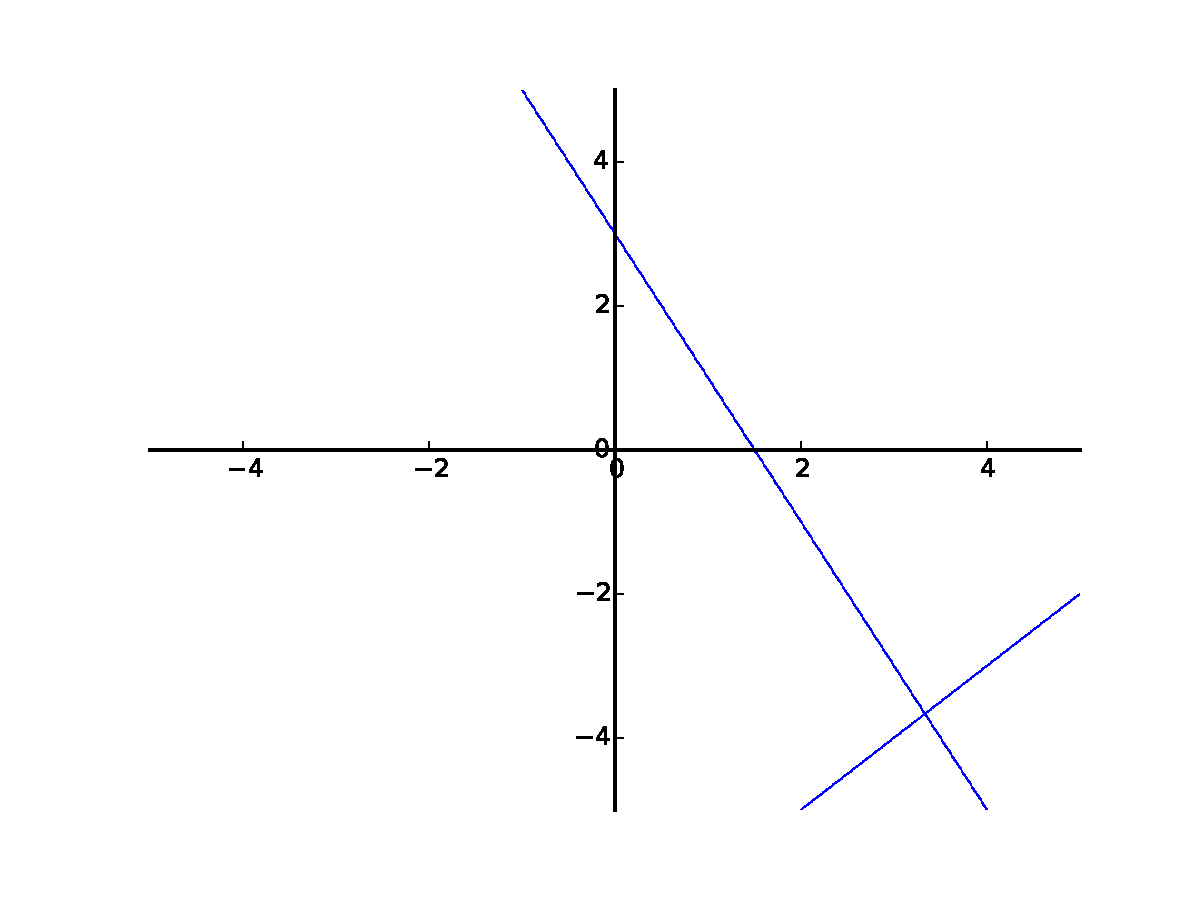
\includegraphics[width=\linewidth]{figs/ex4a.pdf}

\textbf{Exercises 1.1 5b}
% ............

\begin{verbatim}
eq1= Eq(12*x + 4*y, 16)
eq2= Eq(8*x + 4*y, 16)

pp1= plot_implicit(eq1)
pp2= plot_implicit(eq2)
pp1.extend(pp2)
pp1.save('figs/ex5b.pdf')
\end{verbatim}

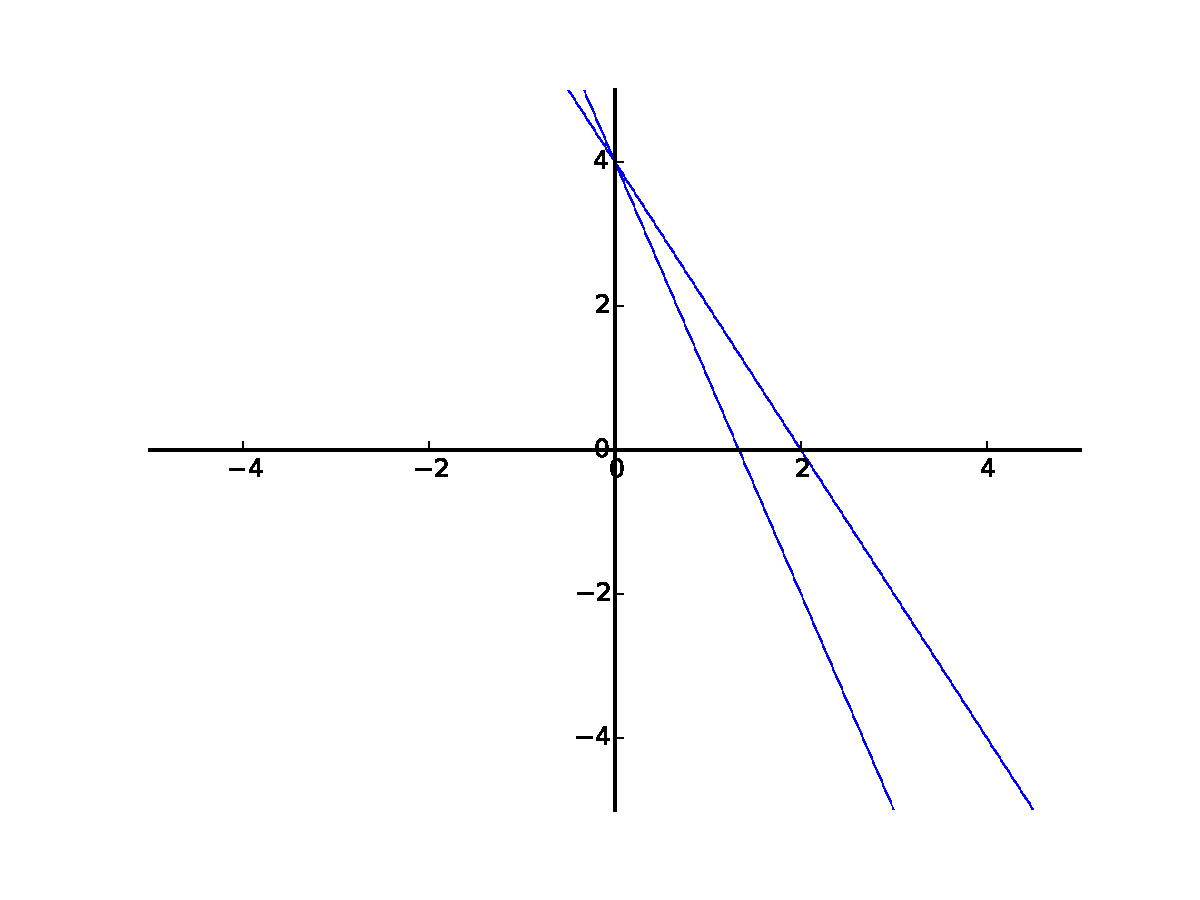
\includegraphics[width=\linewidth]{figs/ex5b.pdf}

\subsection{Solve by row echelon form}
% ------------------------------------

Given a linear system of equations, the solutions can be found by Gaussian
elimination:

\begin{itemize}
\item Extract the coefficients and constants from the equations and put them in
an augmented matrix.
\item Transform the augmented matrix in reduced row echelon form (rref). This is
the result of the Gaussian elimination process.
\item The last columns of the rref matrix lists the solutions of the linear system.
\end{itemize}

Reminder: rref means that every leading coefficient is 1 and is the only nonzero
entry in its column \footnote{http://en.wikipedia.org/wiki/Row\_echelon\_form}. 

\subsubsection{Exercises 1.2 2a}

\begin{equation}\label{eq:na}
\begin{matrix}x + 2 y + 3 z = 12\\2 x - y + 5 z = 3\\3 x + 3 y + 6 z = 21\end{matrix}
\end{equation}

\begin{verbatim}
eq1= Eq(x + 2*y + 3*z, 12)
eq2= Eq(2*x - y + 5*z, 3)
eq3= Eq(3*x + 3*y + 6*z, 21)
\end{verbatim}

Represent the linear systen as \textit{augmented} matrix, where the last column
holds the constants:

\begin{equation}\label{eq:na}
M= \left[\begin{matrix}1 & 2 & 3 & \textit{12}\\
                       2 & -1 & 5 & \textit{3}\\
                       3 & 3 & 6 & \textit{21}\end{matrix}\right]
\end{equation}

In \sympy use the \href{http://docs.sympy.org/latest/modules/polys/reference.html#sympy.polys.polytools.Poly}{\texttt{Poly}}
class to conveniently extract the coefficients at the left hand side of
the equations:

\begin{verbatim}
M= Matrix([
    Poly(eq1.lhs).coeffs(),
    Poly(eq2.lhs).coeffs(),
    Poly(eq3.lhs).coeffs()
])
const= Matrix([eq1.rhs, eq2.rhs, eq3.rhs])
M= const.col_insert(0, M)
\end{verbatim}

In reduced row echelon form, with indexes of the pivot variables on the right:

\begin{equation}\label{eq:na}
RREF= \begin{pmatrix}\left[\begin{matrix}1 & 0 & 0 & 1\\0 & 1 & 0 & 4\\0 & 0 & 1 & 1\end{matrix}\right], & \begin{bmatrix}0, & 1, & 2\end{bmatrix}\end{pmatrix}
\end{equation}

Solutions can be read from last column of the RREF $\left[\begin{matrix}x:1\\y:4\\z:1\end{matrix}\right]$. Verify the solutions solve
the initial system of equations:

\begin{verbatim}
rref= M.rref()
sols= rref[0].col(-1)

eq1.subs({x:sols[0], y:sols[1], z:sols[2]}) # True
eq2.subs({x:sols[0], y:sols[1], z:sols[2]}) # True
eq3.subs({x:sols[0], y:sols[1], z:sols[2]}) # True

# Or the same returning dict {x: 1, y: 4, z: 1}
solve([eq1, eq2, eq3]) 
\end{verbatim}

\subsubsection{Exercises 1.2 3d}
% ..............................

Linear system:

\begin{equation}\label{eq:na}
\begin{matrix}
    - 2 x + 3 y - 2 z = 8 \\
    - x + 2 y - 10 z = 0 \\
    5 x - 7 y + 4 z = -20
\end{matrix}
\end{equation}

Augmented matrix:

\begin{equation}\label{eq:na}
\left[\begin{matrix}-2 & 3 & -2 & 8\\-1 & 2 & -10 & 0\\5 & -7 & 4 & -20\end{matrix}\right]
\end{equation}

Reduced row echelon form with solutions in the last column:

\begin{equation}\label{eq:na}
\begin{pmatrix}\left[\begin{matrix}1 & 0 & 0 & -3 \\
                                   0 & 1 & 0 & 1 \\
                                   0 & 0 & 1 &
\frac{1}{2}\end{matrix}\right], & \begin{bmatrix}0, & 1, & 2\end{bmatrix}\end{pmatrix}
\end{equation}

In \sympy:

\begin{verbatim}
eq1= Eq(-2*x + 3*y -2*z, 8)
eq2= Eq(-x + 2*y - 10*z, 0)
eq3= Eq(5*x - 7*y + 4*z, -20)

M= Matrix([
    Poly(eq1.lhs).coeffs(),
    Poly(eq2.lhs).coeffs(),
    Poly(eq3.lhs).coeffs()
])
const= Matrix([eq1.rhs, eq2.rhs, eq3.rhs])
M= const.col_insert(0, M)
rref= M.rref()
sols= rref[0].col(-1)

# Checked: {x: -3, y: 1, z: 1/2}
solve([eq1, eq2, eq3])
\end{verbatim}

\subsection{Vector arithmetic}
% ----------------------------

\subsubsection{Exercise 1.3.1}

Given two vectors:

\begin{verbatim}
va= Matrix([2, 0])
vb= Matrix([2, 1])
\end{verbatim}

plot the results of the operations 

\subsubsection{(a-e)}

\begin{verbatim}
vA= va + vb          # [4 1]
vB= va - vb          # [0 -1]
vC= 3 * va           # [6 0]
vD= -1/2 * vb        # [-1 -0.5]
vE= 3*va - 1/2 * vb  # [5 -0.5]
\end{verbatim}

And plot vectors

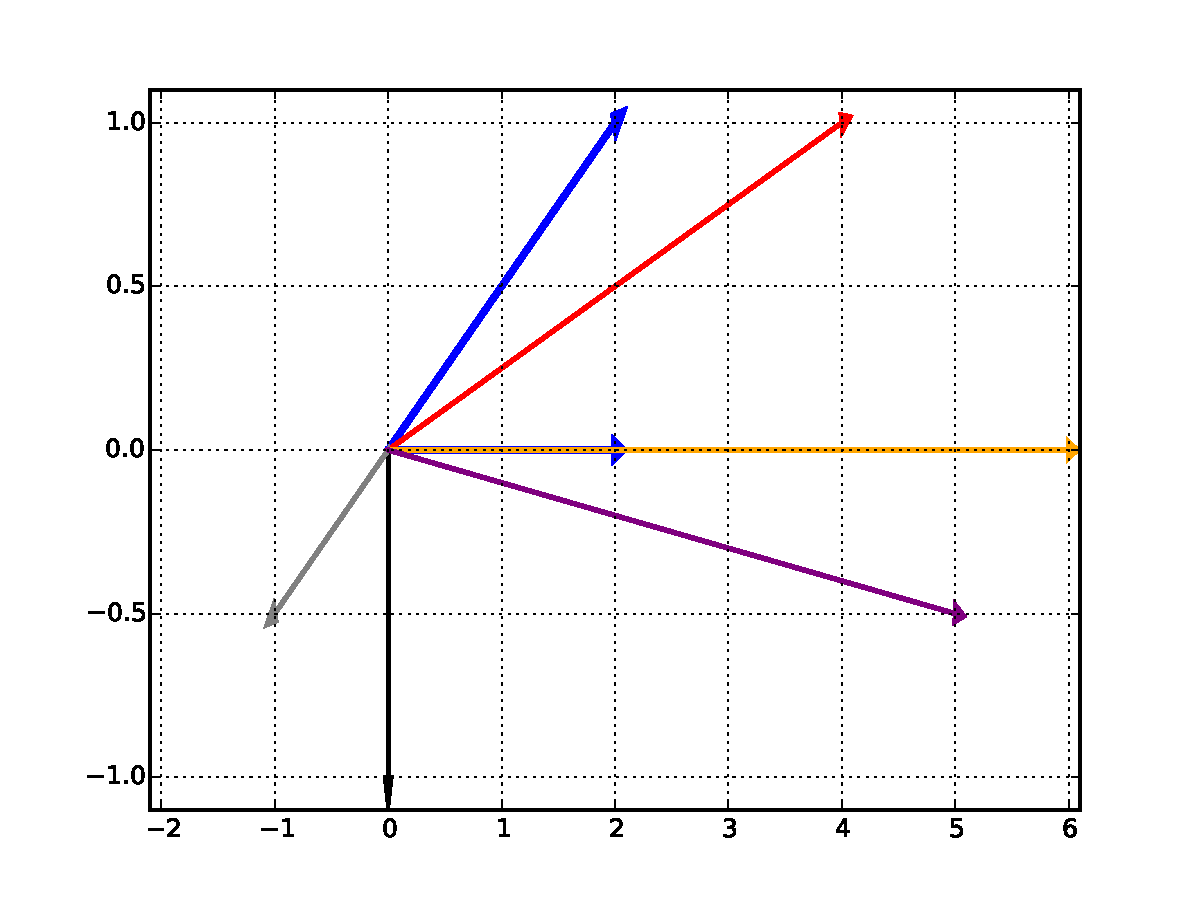
\includegraphics[width=\linewidth]{figs/ex1_3.pdf}

\begin{verbatim}
plt.arrow(0, 0, float(va[0]), float(va[1]), lw= 3, color= 'b', head_width=0.05)
plt.arrow(0, 0, float(vb[0]), float(vb[1]), lw= 3, color= 'b', head_width=0.05)
plt.arrow(0, 0, float(vA[0]), float(vA[1]), lw= 2, color= 'r', head_width=0.05)
plt.arrow(0, 0, float(vB[0]), float(vB[1]), lw= 2, color= 'black', head_width=0.05)
plt.arrow(0, 0, float(vC[0]), float(vC[1]), lw= 2, color= 'orange', head_width=0.05)
plt.arrow(0, 0, float(vD[0]), float(vD[1]), lw= 2, color= 'grey', head_width=0.05)
plt.arrow(0, 0, float(vE[0]), float(vE[1]), lw= 2, color= 'purple', head_width=0.05)
plt.xlim(-2.1, 6.1)
plt.ylim(-1.1, 1.1)
plt.grid()
plt.savefig('figs/ex1_3.pdf')
plt.close()
\end{verbatim}

\subsubsection{Exercise 1.3.8}
% ............................
Show that $x\mathbf{u} + y\mathbf{v} = \mathbf{w}$ where
$\mathbf{u}= (1\ 0)^{T}$, $\mathbf{v}= (0\ 1)^{T}$, and $\mathbf{w}= (x\ y)^{T}$.

This is a consequence of $x(1\ 0) = (x\ 0)$ and $y(0\ 1) = (y\ 0)$. So that
$(x\ 0) + (0\ y) = (x\ y)$

\begin{verbatim}
x, y= symbols('x y')
u= Matrix([1, 0])
v= Matrix([0, 1])
w= Matrix([x, y])
Eq(x*u + y*v, w) # True
\end{verbatim}

\subsubsection{Exercise 1.3.12}
% .............................

Find the real numbers x, y and z, if

\begin{equation}\label{eq:na}
\left[\begin{matrix}x - 2 z\\2 x + y\\- y + 6 z\end{matrix}\right] = \left[\begin{matrix}5\\3\\17\end{matrix}\right]
\end{equation}

Which is solved for:

\begin{equation}\label{eq:}
sols= \begin{bmatrix}\begin{Bmatrix}x : 7, & y : -11, & z : 1\end{Bmatrix}\end{bmatrix}
\end{equation}

\begin{verbatim}
eq1= Eq(x * Matrix([1, 2, 0]) + y * Matrix([0, 1, -1]) + z * Matrix([-2, 0, 6]),
    Matrix([5, 3, 17]))
sols= solve(eq1)
\end{verbatim}

\subsubsection{Exercise 1.3.12}
% .............................

Show that vectors \textbf{u} and \textbf{v} in space $\mathbb{R}^n$ can be
$\mathbf{u} \cdot{} \mathbf{v} = \mathbf{0}$ even if neither \textbf{u} or \textbf{v}
are 0 vectors.

Set:

\begin{verbatim}
u= Matrix([-1, 1])
v= Matrix([1, 1])
u.dot(v) == 0 # True
\end{verbatim}

\subsection{Arithmetic of Matrices}
% ---------------------------------

\subsubsection{Exercise 1.4.1}
% .............................

Given matrix \textbf{B}, note that $3\mathbf{B} = \mathbf{B} + \mathbf{B} + \mathbf{B}$

\begin{equation}
\left[\begin{matrix}6 & -1\\5 & 3\end{matrix}\right]
\end{equation}

\begin{verbatim}
B= Matrix([[6, -1], [5, 3]])
3*B == (B + B + B)
\end{verbatim}

\subsubsection{Exercise 1.4.6}
% .............................

Note how matrx multiplication can result in zero matrix:

\begin{equation}
\left[\begin{matrix}5 & -1 & -2\\10 & -2 & -4\\15 & -3 & -6\end{matrix}\right]
\left[\begin{matrix}1 & 1 & 3\\1 & -1 & -1\\2 & 3 & 8\end{matrix}\right]
= \left[\begin{matrix}0 & 0 & 0\\0 & 0 & 0\\0 & 0 & 0\end{matrix}\right]
\end{equation}

\begin{verbatim}
A= Matrix(3, 3, [5, -1, -2, 10, -2, -4, 15, -3, -6])
B= Matrix(3, 3, [1, 1, 3, 1, -1, -1, 2, 3, 8])
Z= A * B
\end{verbatim}

\subsubsection{Exercise 1.4.8}
% ............................

$\mathbf{x}_n = \mathbf{A}^n\mathbf{x}$ Describes a \textbf{discrete dynamical
system}. Apply this formula to

\begin{equation}\label{eq:ex148}
A = \left[\begin{matrix}0.5 & 0.5\\0.5 & 0.5\end{matrix}\right]
\end{equation}

\begin{verbatim}
A= Matrix(2, 2, [1/2, 1/2, 1/2, 1/2])
\end{verbatim}

For the matrix in \ref{eq:ex148} $A^n = A$:

\begin{verbatim}
A**2 == A # True
A**3 == A # True
A**10 == A # True
\end{verbatim}

matrix in \ref{eq:ex148} is a Markov matrix since the colum sums equal 1.

\subsubsection{Exercise 1.4.10}
% .............................

Determine the image of the matrix \textbf{F} after transformation \textbf{AF}:

\begin{equation}
A = \left[\begin{matrix}1 & 0.2\\0 & 1\end{matrix}\right]
\end{equation}

\begin{equation}
F = \left[\begin{matrix}1 & 1 & 2 & 2 & 1.4 & 1.4 & 2 & 2 & 1.4 & 1.4\\1 & 3 & 3 & 2.6 & 2.6 & 2 & 2 & 1.6 & 1.6 & 1\end{matrix}\right]
\end{equation}

\begin{equation}\label{eq:}
AF = \left[\begin{matrix}1.2 & 1.6 & 2.6 & 2.52 & 1.92 & 1.8 & 2.4 & 2.32 & 1.72 & 1.6\\1 & 3 & 3 & 2.6 & 2.6 & 2 & 2 & 1.6 & 1.6 & 1\end{matrix}\right]
\end{equation}

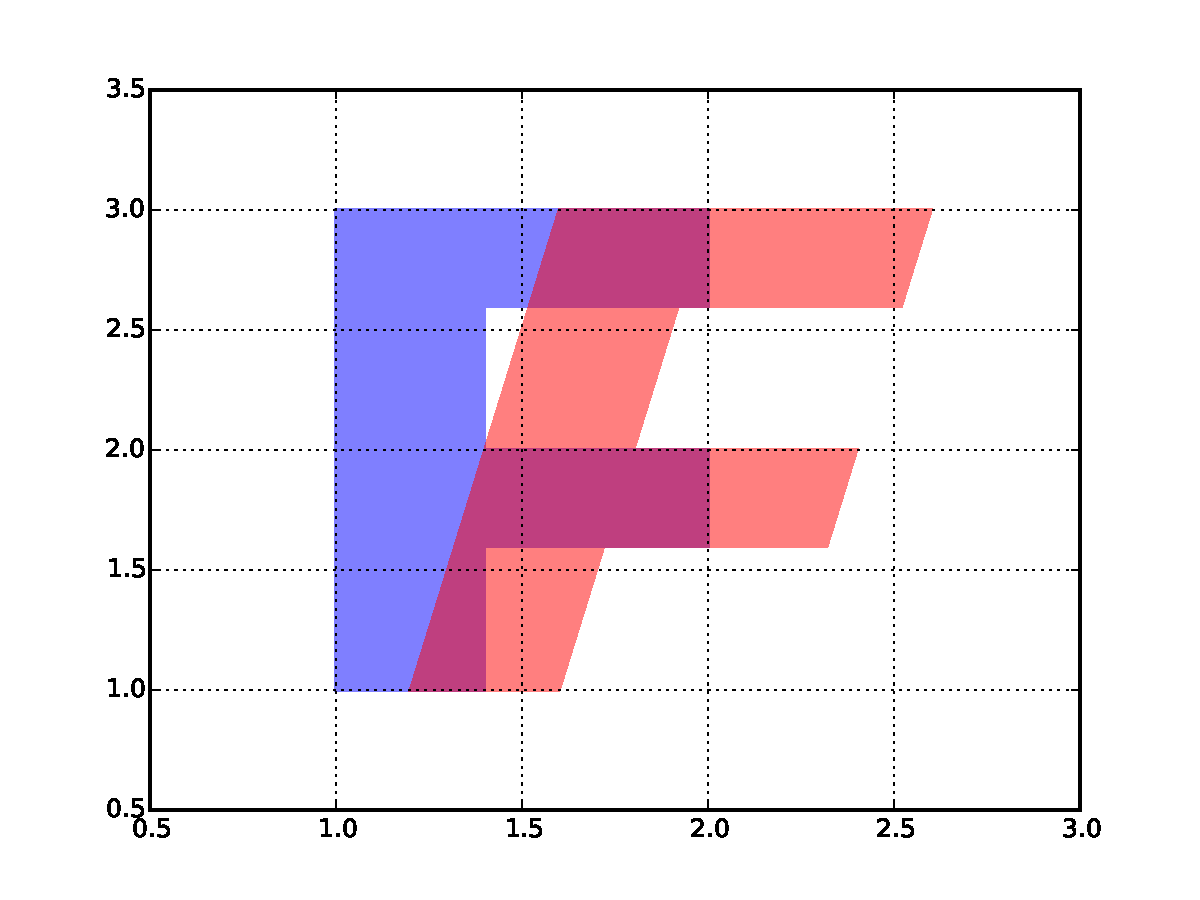
\includegraphics[width=\linewidth]{figs/1_4_10.pdf}

This is showing that the matrix operation $\mathbf{AF} = \mathbf{F_2}$ can be seen as
$\mathbf{f(F)}= \mathbf{F_2}$. That is, the matrix on the left-hand (\textbf{A})
side acts like a function that transforms its argument (\textbf{F}).

\begin{verbatim}
A= Matrix([[1, 0.2], [0, 1]])
F= Matrix([
    [1, 1, 2, 2, 1.4, 1.4, 2, 2, 1.4, 1.4],
    [1, 3, 3, 2.6, 2.6, 2, 2, 1.6, 1.6, 1]])

AF= A*F

verts_F= []
for i in range(F.cols):
    verts_F.append((F[0, i], F[1, i]))
verts_AF= []
for i in range(AF.cols):
    verts_AF.append((AF[0, i], AF[1, i]))

fig = plt.figure()
ax = fig.add_subplot(1, 1, 1)
poly_F = patches.Polygon(verts_F, color= 'b', alpha= 0.5)
poly_AF = patches.Polygon(verts_AF, color= 'r', alpha= 0.5)
ax.set_xlim((0.5, 3))
ax.set_ylim((0.5, 3.5))
ax.add_patch(poly_F)
ax.add_patch(poly_AF)
plt.grid()
plt.savefig('figs/1_4_10.pdf')
\end{verbatim}

\subsubsection{Exercise 1.4.11}
% .............................

\begin{verbatim}
O= Matrix.zeros(2, 1)
X= Matrix([x, y])
\end{verbatim}

\begin{verbatim}
A= Matrix([[1, 2], [3, 5]])
xy= A.solve(O) # x:0, y:0
# Or
xy= A.LUsolve(O) 
# Or
solve(A*X)

A= Matrix([[2, 7], [3, 15]]) # x:0, y:0
xy= A.solve(O)

A= Matrix([[1, 4], [3, 12]]) # Linearly dependent!
xy= A.solve(O)
>>> ValueError: Matrix det == 0; not invertible.
\end{verbatim}

\subsubsection{Exercise 1.4.12}
% .............................

Determine whether vector \textbf{w} is a linear combination of vector \textbf{u}
and \textbf{v}.

Effectively this is asking if the equation $x\mathbf{u} + y\mathbf{v} = \mathbf{w}$
can be resolved.


\begin{itemize}
\item Create an augmented matrix as [u, v, w].
\item Transform the augmented matrix in row echelon form.
\item Get coefficients x and y from last column of RREF. The three vectors are linearly
independent and \textbf{w} $\neq$ \textbf{u} + \textbf{v} (\textbf{w} is not a linear
combination of \textbf{u} and \textbf{v}).

\end{itemize}

\begin{verbatim}
w= Matrix(2, 1, [1, 0])
u= Matrix(2, 1, [5, 8])
v= Matrix(2, 1, [2, 4])
A=  w.col_insert(0, v).col_insert(0, u)
A.rref()
\end{verbatim}

\begin{equation}
REF= \begin{pmatrix}\left[\begin{matrix}1 & 0 & 1\\0 & 1 & -2\end{matrix}\right], & \begin{bmatrix}0, & 1\end{bmatrix}\end{pmatrix}
\end{equation}

\textbf{w} is a linear combination. In fact $1\mathbf{u} -2\mathbf{v}= \mathbf{w}$

\begin{verbatim}
w= Matrix(2, 1, [0, 1])
u= Matrix(2, 1, [5, 8])
v= Matrix(2, 1, [2, 4])
A=  w.col_insert(0, v).col_insert(0, u)
A.rref()
\end{verbatim}

\begin{equation}\label{eq:}
\begin{pmatrix}\left[\begin{matrix}1 & 0 & - \frac{1}{2}\\0 & 1 & \frac{5}{4}\end{matrix}\right], & \begin{bmatrix}0, & 1\end{bmatrix}\end{pmatrix}
\end{equation}

\begin{verbatim}
w= Matrix(3, 1, [1, 2, 3])
u= Matrix(3, 1, [1, 0, 0])
v= Matrix(3, 1, [0, 1, 0])
A=  w.col_insert(0, v).col_insert(0, u)
A.rref()
\end{verbatim}

\begin{equation}
REF= \begin{pmatrix}\left[\begin{matrix}1 & 0 & 0\\0 & 1 & 0\\0 & 0 & 1\end{matrix}\right], & \begin{bmatrix}0, & 1, & 2\end{bmatrix}\end{pmatrix}
\end{equation}

\textbf{w} cannot be a linear combination. In fact
$0\mathbf{u} + 0\mathbf{v} \neq [1\ 2\ 3]^T$

\begin{verbatim}
w= Matrix(3, 1, [1, 2, 3])
u= Matrix(3, 1, [4, 8, 0])
v= Matrix(3, 1, [1, 2, -3/7])
A=  w.col_insert(0, v).col_insert(0, u)
A.rref()
\end{verbatim}

\begin{equation}\label{eq:}
\begin{pmatrix}\left[\begin{matrix}1 & 0 & 2.0\\0 & 1.0 & -7.0\\0 & 0 & 0\end{matrix}\right], & \begin{bmatrix}0, & 1\end{bmatrix}\end{pmatrix}
\end{equation}

\subsection{Matrix Algebra}
% -------------------------

\subsubsection{Exrcises 1.5.2}
% ............................

Given $A = \left[\begin{matrix}5 & -1 & -2\\1 & -3 & 2\end{matrix}\right]$

A) Find \textbf{B} suc that \textbf{A} + \textbf{B} = \textbf{O} with \textbf{O}
a 2 x 3 matrix.

Requires $\mathbf{A} = \mathbf{B} \Rightarrow \mathbf{B} = -\mathbf{A}$

\begin{verbatim}
A= Matrix([[5, -1, -2], [1, -3, 2]])
O= Matrix.zeros(2, 3)
\end{verbatim}


\subsubsection{Exrcises 1.5.7}
% ----------------------------

Determine the scalar $\lambda$ so that $\mathbf{Ax} = \lambda \mathbf{x}$ with
$\mathbf{A} = \left[\begin{matrix}2 & 1 \\ 1 & 2\end{matrix}\right]$ and $\mathbf{x} = \left[\begin{matrix} 1\\1 \end{matrix}\right]$

$\lambda = 3$ since $\mathbf{Ax} = [3\ 3]^T$.

\begin{verbatim}
A= Matrix([[2, 1], [1, 2]])
x= Matrix(2, 1, [1, 1])
l= symbols('lambda')
solve(Eq(A*x, l*x)) # Lambda= 3
\end{verbatim}

\subsubsection{Exrcises 1.5.10}
% ----------------------------

Given \textbf{T} a transition matrix from a Markov chain and \textbf{p} a
probability vector. Note that the probility vector must sum to 1.

What is the probility that the chain is in a given state after $k$ steps?

The answer is given by $\mathbf{p}_k = \mathbf{T}^k\mathbf{p}$.

For:
\begin{equation}
\left[\begin{matrix}0.6 & 0.7\\0.4 & 0.3\end{matrix}\right]
\end{equation}

\begin{equation}
\left[\begin{matrix}0.5\\0.5\end{matrix}\right]
\end{equation}

Determine $\mathbf{p}_k$ for $k$ in 1, 2, 10, 100, 100000:

$p_{k= 1} = \left[\begin{matrix}0.65\\0.35\end{matrix}\right]$

$p_{k= 2} = \left[\begin{matrix}0.635\\0.365\end{matrix}\right]$

$p_{k= 10} = \left[\begin{matrix}0.63636363635\\0.36363636365\end{matrix}\right]$

$p_{k= 100} = \left[\begin{matrix}0.636363636363634\\0.363636363636362\end{matrix}\right]$

$p_{k= 100000} = \left[\begin{matrix}0.636363636361267\\0.36363636363501\end{matrix}\right]$

Note how the probability vector converges in the long period. The probability vector
at the initial state $k = 0$ might represent the proportion of different species
in the environment. Given the probility of change in \textbf{T}, we can ask the question:
What proportion of species we will see after $k$ iterations (\textit{e.g} generations)?

\begin{verbatim}
T= Matrix(2,2, [0.6, 0.7, 0.4, 0.3])
p= Matrix(2, 1, [0.5, 0.5])
ks= [1, 2, 10, 100, 100000]

for k in ks:
    p_k= T**k * p
    print latex(p_k)
\end{verbatim}


\subsection{Type of solutions}
% ========================================

\subsubsection{Exrcises 1.7.8}
% ----------------------------

\begin{equation}\label{eq:}
\textbf{M} = \left[\begin{matrix}1 & 1 & 1 & 0 & 0 & 0 & 6\\0 & 0 & 0 & 1 & 1 & 1 & 15\\1 & 0 & 0 & 1 & 0 & 0 & 5\\0 & 1 & 0 & 0 & 1 & 0 & 7\\0 & 0 & 1 & 0 & 0 & 1 & 9\end{matrix}\right]
\end{equation}

\begin{equation}\label{eq:}
\mathbf{M_{rref}}= \begin{pmatrix}\left[\begin{matrix}1 & 0 & 0 & 0 & -1 & -1 & -10\\0 & 1 & 0 & 0 & 1 & 0 & 7\\0 & 0 & 1 & 0 & 0 & 1 & 9\\0 & 0 & 0 & 1 & 1 & 1 & 15\\0 & 0 & 0 & 0 & 0 & 0 & 0\end{matrix}\right], & \begin{bmatrix}0, & 1, & 2, & 3\end{bmatrix}\end{pmatrix}
\end{equation}

There are six variables with coefficents arranged as in matrix $\mathbf{M}$. In
RREF it appears the first four variables, $x_1$ to $x_4$, have 1 as leading
coefficient, as reported by \sympy in the list of pivot variables indexes on the right
(0, 1, 2, 3). Variables $x_5$ and $x_6$ are \textit{free} with coefficients given
in the respective columns. The solutions are therefore:

\begin{equation}\label{eq:}
\begin{Bmatrix}x_{1} : x_{5} + x_{6} - 10, & x_{2} : - x_{5} + 7, & x_{3} : - x_{6} + 9, & x_{4} : - x_{5} - x_{6} + 15\end{Bmatrix}
\end{equation}

\begin{verbatim}
M= Matrix([
[1, 1, 1, 0, 0, 0, 6],
[0, 0, 0, 1, 1, 1, 15],
[1, 0, 0, 1, 0, 0, 5],
[0, 1, 0, 0, 1, 0, 7],
[0, 0, 1, 0, 0, 1, 9],
])
M_rref= M.rref()
\end{verbatim}

Solve system of equations:

\begin{verbatim}
x1, x2, x3, x4, x5, x6= symbols('x1:7')
r1= Eq(x1 + x2 + x3, 6)
r2= Eq(x4 + x5 + x6, 15)
r3= Eq(x1 + x4, 5)
c1= Eq(x2 + x5, 7)
c2= Eq(x3 + x6, 9)
sols= solve([r1, r2, r3, c1, c2])
\end{verbatim}

\subsubsection{Exrcises 1.7.11}
% ----------------------------

\begin{verbatim}
x, y, z, t= symbols('x y z t', real= True)

eq1= Eq(2*x - 4*y + 4*z + 0.077*t, 3.86)
eq2= Eq(     -2*y + 2*z - 0.056*t, -3.47)
eq3= Eq(2*x - 2*y,                 0)
sols= solve([eq1, eq2, eq3], [x, y, z])
\end{verbatim}

The solutions \texttt{sols}  are in \ref{eq:ex1_7_11}.

Solving via augmented matrix in reduced row echelon form:

\begin{verbatim}
M= Matrix([
    [2, -4, 4, 0.077, 3.86],
    [0, -2, 2, -0.056, -3.47],
    [2, -2, 0, 0, 0]
])
M_rref= M.rref()
\end{verbatim}

\begin{equation}\label{eq:}
\begin{matrix}
2 x - 4 y + 4 z + 0.077 t= 3.86, & \\
- 2 y + 2 z - 0.056 t = -3.47, & \\
2 x - 2 y = 0\end{matrix}
\end{equation}

\begin{equation}\label{eq:}
M= \left[\begin{matrix}2 & -4 & 4 & 0.077 & 3.86\\0 & -2 & 2 & -0.056 & -3.47\\2 & -2 & 0 & 0 & 0\end{matrix}\right]
\end{equation}

\begin{equation}\label{eq:}
M_{rref} = \begin{pmatrix}\left[\begin{matrix}1 & 0 & 0 & 0.0945 & 5.4\\0 & 1 & 0 & 0.0945 & 5.4\\0 & 0 & 1 & 0.0665 & 3.665\end{matrix}\right], & \begin{bmatrix}0, & 1, & 2\end{bmatrix}\end{pmatrix}
\end{equation}

Note that the 4th column holds the coefficients for the free variable $t$ while the
last column has the values for $x, y, z$. Compare to the solutions
from \sympy \texttt{solve}:

\begin{equation}\label{eq:ex1_7_11}
\begin{Bmatrix}x : - 0.0945 t + 5.4, & y : - 0.0945 t + 5.4, & z : - 0.0665 t + 3.665\end{Bmatrix}
\end{equation}

\subsection{The inverse matrix method}
% ====================================

\subsubsection{Exrcises 1.8.3}
% ----------------------------

What effect has the matrix \textbf{E} on the matrix \textbf{A}. With \textbf{A}
a generic 3x3 matrix:

\begin{verbatim}
x1, x2, x3, x4, x5, x6, x7, x8, x9= symbols('x1:10')
k= symbols('k', zero= False)
A= Matrix(3,3, [x1, x2, x3, x4, x5, x6, x7, x8, x9])
\end{verbatim}

\begin{equation}\label{eq:1_8_3A}
\mathbf{A} = \left[\begin{matrix}x_{1} & x_{2} & x_{3}\\x_{4} & x_{5} & x_{6}\\x_{7} & x_{8} & x_{9}\end{matrix}\right]
\end{equation}

\begin{equation}\label{eq:}
\mathbf{E} = \left[\begin{matrix}1 & 0 & 0\\0 & -1 & 0\\0 & 0 & 1\end{matrix}\right]
\end{equation}

\begin{verbatim}
E_a= Matrix([
    [1, 0, 0],
    [0, -1, 0],
    [0, 0, 1]
])
print latex(E_a * A)
\end{verbatim}

\begin{equation}\label{eq:}
\mathbf{E_aA} = \left[\begin{matrix}x_{1} & x_{2} & x_{3}\\- x_{4} & - x_{5} & - x_{6}\\x_{7} & x_{8} & x_{9}\end{matrix}\right]
\end{equation}

\begin{verbatim}
E_b= Matrix([
    [0, 0, 1],
    [0, 1, 0],
    [1, 0, 0]
])
print latex(E_b * A)
\end{verbatim}

\begin{equation}\label{eq:}
\mathbf{E_bA} = \left[\begin{matrix}x_{7} & x_{8} & x_{9}\\x_{4} & x_{5} & x_{6}\\x_{1} & x_{2} & x_{3}\end{matrix}\right]
\end{equation}

\begin{verbatim}
E_c= Matrix([
    [k, 0, 0],
    [0, 1, 0],
    [0, 0, 1]
])
print latex(E_c * A)
\end{verbatim}

\begin{equation}\label{eq:}
\mathbf{E_cA} = \left[\begin{matrix}k x_{1} & k x_{2} & k x_{3}\\x_{4} & x_{5} & x_{6}\\x_{7} & x_{8} & x_{9}\end{matrix}\right]
\end{equation}


\begin{verbatim}
E_d= Matrix([
    [1, 0, 0],
    [0, 1, 0],
    [0, 0, -1/k]
])
print latex(E_d * A)
\end{verbatim}

\begin{equation}\label{eq:}
\mathbf{E_dA} = \left[\begin{matrix}x_{1} & x_{2} & x_{3}\\x_{4} & x_{5} & x_{6}\\- \frac{x_{7}}{k} & - \frac{x_{8}}{k} & - \frac{x_{9}}{k}\end{matrix}\right]
\end{equation}

\subsubsection{Exrcises 1.8.5}
% ----------------------------

Solve the linear systems using inverse matrix method.

\begin{equation}\label{eq:eqs_1_8_5}
\begin{matrix}x + 2 y = 3, & \\ - x + 4 y = 5\end{matrix}
\end{equation}

The coefficients on the LHS of the equations can be thought as a matrix
\textbf{A}. \textbf{A} transforms the vector of unknown coefficients \textbf{x}
to produce the vector of constants \textbf{b} on the RHS:

\begin{equation}\label{eq:1_8_5}
\mathbf{A}\mathbf{x} = \mathbf{b}
\end{equation}

To find the vector \textbf{x} we can rearrange \ref{eq:eqs_1_8_5} as:

\begin{equation}
\mathbf{x} = \mathbf{A}^{-1}\mathbf{b}
\end{equation}

In case of \ref{eq:eqs_1_8_5} we have $\mathbf{A} = \left[\begin{matrix}1 & 2\\-1 & 4\end{matrix}\right]$,
$\mathbf{b} = \left[\begin{matrix}3\\5\end{matrix}\right]$. So
$\mathbf{A^{-1}} = \left[\begin{matrix}\frac{2}{3} & - \frac{1}{3}\\\frac{1}{6} & \frac{1}{6}\end{matrix}\right]$
and $\mathbf{x} = \mathbf{A^{-1}b} = \left[\begin{matrix}\frac{1}{3}\\\frac{4}{3}\end{matrix}\right]$

\begin{verbatim}
x, y= symbols('x y')
eq1= Eq(x + 2*y, 3)
eq2= Eq(-x + 4*y, 5)

A = Matrix(2, 2, [1, 2, -1, 4])
b = Matrix(2, 1, [3, 5])
Ai= A.inv()
x= Ai * b
\end{verbatim}

In case of $\mathbf{Ax = b}$ as:

\begin{equation}\label{eq:}
\left[\begin{matrix}1 & 0 & 2\\2 & 3 & 1\\3 & 6 & 0\end{matrix}\right]
\mathbf{x} = 
\left[\begin{matrix}-1\\1\\9\end{matrix}\right]
\end{equation}

Matrix \textbf{A} is not invertible and the system has no solutions.

\begin{verbatim}
A = Matrix([
[1, 0, 2],
[2, 3, 1],
[3, 6, 0]
])
b= Matrix(3, 1,  [-1 , 1, 9])

Ai= A.inv()
# ValueError: Matrix det == 0; not invertible.
\end{verbatim}

\subsubsection{Exrcises 1.8.7}
% ----------------------------

\textbf{Leontief input-output model}. Represents the production \textbf{p} and
demand \textbf{d} as a matrix. \textbf{p} and \textbf{d} are vectors where each entry
represents a good. The production of goods is represented as a matrix where each row
states how much units of the other goods (input) is required to produce one unit
of that good (output). With this model we can ask how much input is needed to produce
a given amount of output.

$$
\bordermatrix{\text{}& O & E & S \cr
                 O & 0.25 &  0.15  & 0.1 \cr
                 E & 0.4  &  0.15  & 0.2 \cr
                 S & 0.15 &  0.2   & 0.2} = \mathbf{A}
$$

Reading this matrix row by row, it tells how much Oil, Energy and Services it is
needed to produce one unit of O, E, or S. For example 1 unit of O requires 0.25 units
of O, 0.15 of E and 0.1 units of S.

From this matrix we can relate the production vector \textbf{p} to the demand
vector \textbf{d} as:

\begin{equation}\label{eq:1_8_7io}
\mathbf{p} = \mathbf{Ap} + \mathbf{d}
\end{equation}


We want to know \textbf{p} given \textbf{A} and the demand vector \textbf{d}.
\emph{I.e.} we want to solve \ref{eq:1_8_7io} \emph{w.r.t.} \textbf{p} by re-arranging
to the form \textbf{Ax = b}.

$$\mathbf{
p - Ap = d
}$$

then use the identity matrix to obtain the solvable form \textbf{Ax = b}:

$$\mathbf{
p(I - A) = d
}$$

Now solve by inverting \textbf{(I - A)}:

$$\mathbf{
p = (I - A)^{-1} d
}$$

If the demand for O, E, and S is $\mathbf{d} = [100, 100, 100]^T$ we need to
produce
$\left[\begin{matrix}O \\ E \\ S \end{matrix}\right] = \left[\begin{matrix}220 \\ 276 \\ 235 \end{matrix}\right]$

\begin{verbatim}
A = Matrix([
[0.25, 0.15, 0.1],
[0.4, 0.15, 0.2],
[0.15, 0.2, 0.2]
])

d= Matrix(3, 1, [100, 100, 100])
ii= eye(A.rows)
p= (ii - A).inv() * d
\end{verbatim}



\subsubsection{Exrcises 1.8.8}
% ----------------------------

Show that if \textbf{A} is invertible then $A^Tx=b$ has a unique solution.

\begin{verbatim}
x1, x2, x3, x4, x5, x6, x7, x8, x9= symbols('x1:10')
A= Matrix(3,3, [x1, x2, x3, x4, x5, x6, x7, x8, x9])

k1, k2, k3= symbols('k1:4')
b= Matrix(3, 1, [k1, k2, k3])

A_rref= A.transpose().solve(b).rref()
\end{verbatim}

\begin{equation}\label{eq:}
\mathbf{A_{rref}} = \begin{pmatrix}\left[\begin{matrix}1\\0\\0\end{matrix}\right], & \begin{bmatrix}0\end{bmatrix}\end{pmatrix}
\end{equation}

\textit{Does it mean there is a unique solution?}
\section{2. Euclidean Space}
% **************************

\subsection{Properties of vectors}
% ================================

Dot product, norm and distances. The dot product of two vectors \textbf{A} and
\textbf{B} can be thought as the prodcut of their magnitude times the angle between
them:

$$\mathbf{A} \cdot \mathbf{B} = \|\mathbf{A}\| \cdot \|\mathbf{B}\|cos(\theta)$$

Since $cos(\pi/2) = 0$, if the two vectors are orthogonal their dot product is
0. For example $\left[\begin{matrix}2\\0\end{matrix}\right] \cdot \left[\begin{matrix}0\\2\end{matrix}\right] = 0$

\subsubsection{Exercise 2.1.1}
% ----------------------------

Evaluate

\begin{verbatim}
import matplotlib.pyplot as plt

u= Matrix(2, 1, [-1, 3])
v= Matrix(2, 1, [2, 1])

plt.text(float(u[0])+0.2, float(u[1]), 'u', fontsize= 30, color= 'r')
plt.text(float(v[0])-0.2, float(v[1]), 'v', fontsize= 30, color= 'r')
plt.arrow(0, 0, float(u[0]), float(u[1]), lw= 3, color= 'b', head_width=0.05)
plt.arrow(0, 0, float(v[0]), float(v[1]), lw= 3, color= 'b', head_width=0.05)
plt.xlim((-1.1, 3.1))
plt.ylim((-1.1, 3.1))
plt.grid()
plt.savefig('figs/ex2_1_1.pdf')
plt.close()
\end{verbatim}

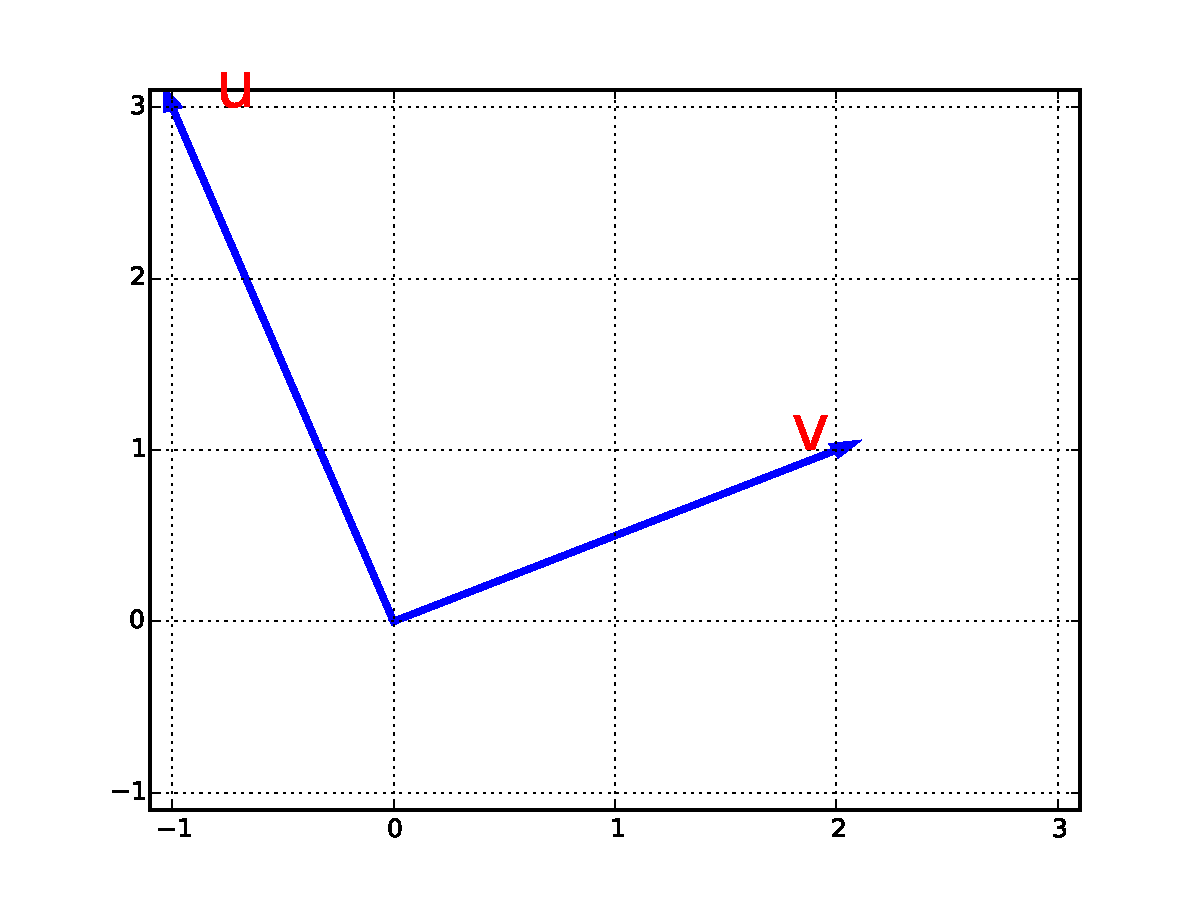
\includegraphics[width=\linewidth]{figs/ex2_1_1.pdf}

\begin{verbatim}
u.dot(v) # 1
v.dot(u) # 1
u.dot(u) # 10
v.dot(v) # 5

u.norm()            # sqrt(10)
u.norm()**2         # 10
v.norm()            # sqrt(5)
v.norm()**2         # 5
(u + v).norm()**2   # 17
(u - v).norm()      # sqrt(13)
\end{verbatim}

\subsubsection{Exercise 2.1.3}
% ----------------------------
Evaluate for
$\mathbf{u} = \left[\begin{matrix}-1\\2\\5\\-3\end{matrix}\right]$ and
$\mathbf{v} = \left[\begin{matrix}2\\-3\\-1\\5\end{matrix}\right]$

\begin{verbatim}
u= Matrix(4, 1, (-1, 2, 5, -3))
v= Matrix(4, 1, (2, -3, -1, 5))
\end{verbatim}

\textbf{Dot product}:

\begin{verbatim}
v.dot(u)    # -28
u.dot(v)    # -28  
v.dot(v)    # 39
u.dot(u)    # 39
\end{verbatim}

Note that commutative property hold. NB \textbf{\texttt{u * v}} raises \texttt{\textcolor{red}{ShapeError: Matrices size mismatch.}}

\textbf{Norm} (\emph{symbol}: $\|u\|$, $\|u + v\|$, $\|u\|^2$, etc)

\begin{verbatim}
u.norm()            # sqrt(39)
u.norm()**2         # 39
v.norm()            # sqrt(39)
v.norm()**2         # 39
(u + v).norm()**2   # 22
\end{verbatim}

\textbf{Distance} $d(u, v) = \| u - v \|$

\begin{verbatim}
(u - v).norm() # sqrt(134)
(v - u).norm() # sqrt(134)
\end{verbatim}

\subsubsection{Exercise 2.1.6}
% ----------------------------

Plot and compute for $\mathbf{u} = \left[\begin{matrix}7\\-2\end{matrix}\right]$
and $\mathbf{v} = \left[\begin{matrix}-5\\3\end{matrix}\right]$

$$\|\mathbf{u} + \mathbf{v} \| = \sqrt{5}$$
and
$$d(\mathbf{u}, \mathbf{v}) = \|\mathbf{u} - \mathbf{v} \| = 13$$

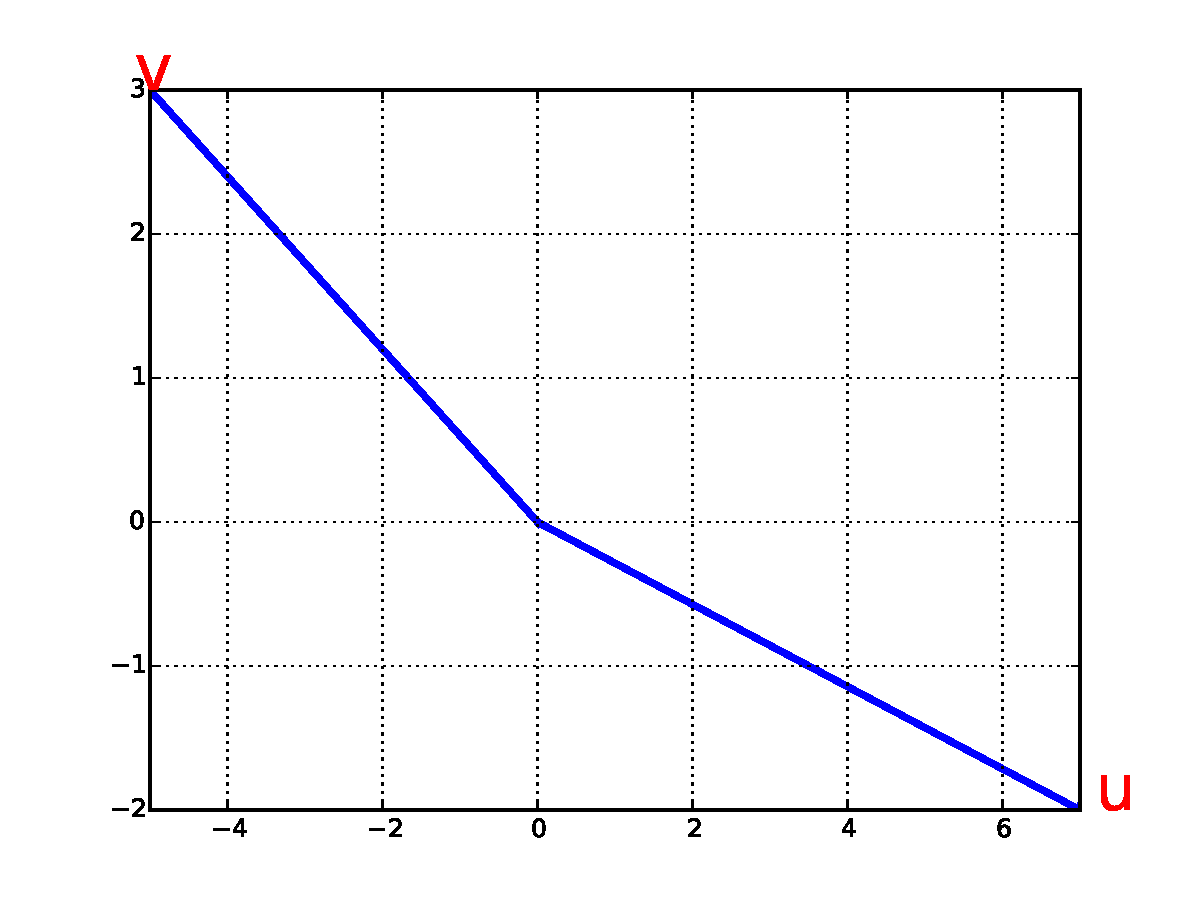
\includegraphics[width=\linewidth]{figs/ex2_1_6.pdf}

\begin{verbatim}
u= Matrix(2, 1, [7, -2])
v= Matrix(2, 1, [-5, 3])

plt.text(float(u[0])+0.2, float(u[1]), 'u', fontsize= 30, color= 'r')
plt.text(float(v[0])-0.2, float(v[1]), 'v', fontsize= 30, color= 'r')
plt.arrow(0, 0, float(u[0]), float(u[1]), lw= 3, color= 'b', head_width=0.05)
plt.arrow(0, 0, float(v[0]), float(v[1]), lw= 3, color= 'b', head_width=0.05)
plt.xlim((-5, 7))
plt.ylim((-2, 3))
plt.grid()
plt.savefig('figs/ex2_1_6.pdf')
plt.close()

(u + v).norm() # sqrt(5)
(u - v).norm() # 13
\end{verbatim}


\subsection{Further Properties of Vectors}
% ========================================

\subsubsection{Exercise 2.2.1}

Find the angle between vectors. The angle is

\begin{equation}\label{eq:uv_angle}
\theta = \arccos(\frac{\mathbf{u} \cdot \mathbf{v}}
{\|\mathbf{u}\| \cdot \|\mathbf{v}\|})
\end{equation}

In \sympy

\begin{verbatim}
def uv_angle(u, v):
    theta= acos(u.dot(v) / (u.norm() * v.norm()))
    return theta
\end{verbatim}

\begin{verbatim}
u= Matrix([1, 1])
v= Matrix([0, 1])
uv_angle(u, v) # pi/4

# As degree:
uv_angle(u, v) * 180/pi # 45

u= Matrix([-1, 2, 3])
v= Matrix([sqrt(2), 1/sqrt(2), -1])
uv_angle(u, v) * 180/pi # ~115 deg
\end{verbatim}

\subsubsection{Exercise 2.2.4}
% ----------------------------
Determine the vector of $k$ so that the vectors are orthogonal to each other.

We want to set the angle between vector equal to 0, \emph{i.e.} Eq. \ref{eq:uv_angle} = 0.

\begin{verbatim}
k= symbols('k', real= True)
u= Matrix([-1, 5, k])
v= Matrix([-3, 2, 7])

eq= Eq(u.dot(v) / (u.norm() * v.norm()) , cos(pi/2))
sol= solve(eq)

# Check
u.subs(k, sol[0]).dot(v) == 0 # True
\end{verbatim}

\subsubsection{Exercise 2.2.6}
% ----------------------------

A vector is normalized by dividing it by its norm. A normalized vector is called
\textbf{unit vector}. In \sympy normlaize with:

\begin{verbatim}
def norm_u(u):
    return u / u.norm()
\end{verbatim}

Determine the value of $k$ so that $\mathbf{\hat{u}} = (1/\sqrt{2}\ 1/2\ k)^T$.

For \textbf{u} to be unit vector, its norm must equal 1. So $\mathbf{\|u\|} = \sqrt{\left\lvert{k}\right\rvert^{2} + 0.75} = 1$.
Solved for $k= \pm 1/2$.

\begin{verbatim}
u= Matrix([1/sqrt(2), 1/2, k])
eq= Eq(u.norm(), 1)
ksol= solve(eq) # [-0.5, 0.5]
\end{verbatim}

\subsubsection{Exercise 2.2.12: Support vector machine}
% -----------------------------------------------------

Find the shortest distance between the vector \textbf{u} and the corresponding
hyperplane. The hyperplane is defined as $\mathbf{v \cdot x} + c = 0$ where
\textbf{v} is a vector of coefficents for the variables in vector \textbf{x} and
$c$ is a constant term. The vector \textbf{u} might represent a data point in
$n$-dimensions.

Remember that an equation in the usual form
$$ax + by +cz + k = 0$$
can be represented in matrix form as
$$ax + by +cz + k
= \left[\begin{matrix}a\\b\\c\end{matrix}\right] \cdot \left[\begin{matrix}x\\y\\z\end{matrix}\right] + k
= \mathbf{v} \cdot \mathbf{x} + k
= 0$$

The shortest distance between \textbf{u} and hyerplane is given by

\begin{equation}\label{eq:ex2_2_12_svm}
d_{shortest} = \frac{|\mathbf{u \cdot v} + c|}{\|\mathbf{v}\|}
\end{equation}

Given \textcolor{red}{$\mathbf{u} = (1\ 1)^T$} and hyperplane \textcolor{blue}{$y= x + 1$}, find the shortes
distance. For this we need to extract the vector of coefficents \textbf{v} from $y= x + 1$, which for convenience can be
re-arranged as $x - y + 1 = 0$.
The coeffients \textbf{v} are $\left[\begin{matrix}1\ \mathit{x} \\ -1\ \mathit{y} \end{matrix}\right]$.

Putting it all together:

\begin{equation}
d_{shortest} = \frac{
    |\left[\begin{matrix}1\\1\end{matrix}\right] \cdot \left[\begin{matrix}1\\-1\end{matrix}\right] + 1|
}{
    \|\left[\begin{matrix}1\\-1\end{matrix}\right]\|
} = \frac{\sqrt{2}}{2} \approx 0.707
\end{equation}

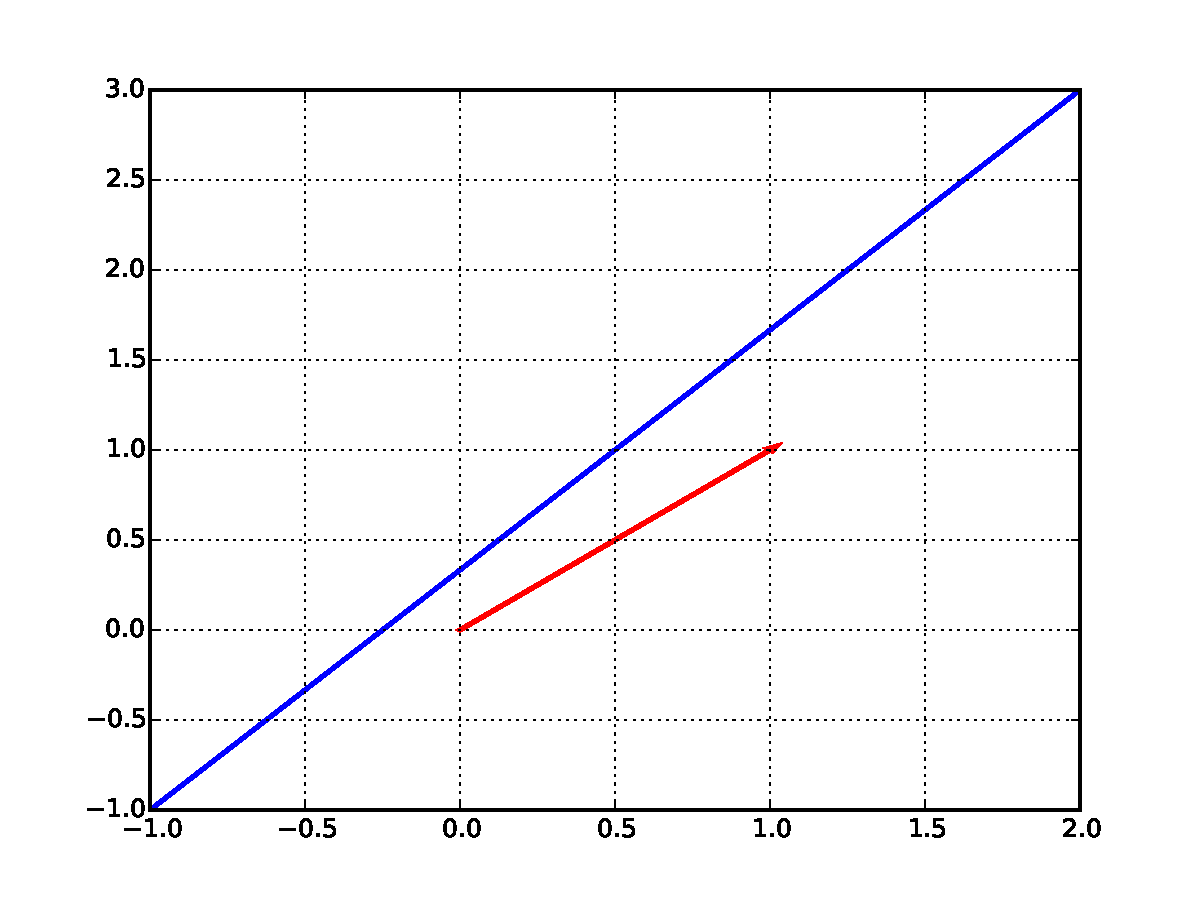
\includegraphics[width=0.75\linewidth]{figs/ex2_2_12_svm.pdf}

\begin{verbatim}
u= Matrix([1, 1])
hyp= Eq(x + 1, y)

# 1. Re-arrange hyp to have x + y + c= 0
hyp2= Eq(hyp.lhs - hyp.rhs)

# 2. Re-arrange in matrix form
cfdict= hyp2.lhs.as_expr().as_coefficients_dict()
v= Matrix([cfdict[x], cfdict[y]])
c= cfdict[numbers.One()]
d_shortest= abs(u.dot(v) + c) / v.norm()
\end{verbatim}

Plotted with:

\begin{verbatim}
plt.plot([-1, 2], [hyp.lhs.subs(x, -2), hyp.lhs.subs(x, 2)], 'b-', lw= 2)
plt.arrow(0, 0, float(u[0]), float(u[1]), lw= 2, color= 'red')
plt.grid()
plt.xlim([-0.5, 1.5])
plt.ylim([-0.5, 1.5])
plt.savefig('figs/ex2_2_12_svm.pdf')
plt.close()
\end{verbatim}

\subsubsection{Exercise 2.2.12d}
% ------------------------------

For $\mathbf{u} = \left[\begin{matrix}1\\2\\3\\4\end{matrix}\right]$ and
$x + 2y + z + w = 10$. We have

$$
d_{shortest}
= \frac{|\mathbf{u} \cdot \mathbf{v} + c|}{\|\mathbf{v}\|}
= \frac{|\left[\begin{matrix}1\\2\\3\\4\end{matrix}\right] \cdot \left[\begin{matrix}1\\2\\1\\1\end{matrix}\right] - 10|}{\|\left[\begin{matrix}1\\2\\1\\1\end{matrix}\right]\|}
= \frac{2 \sqrt{7}}{7}
\approx 0.76
$$

\begin{verbatim}
x,y,z,w = symbols('x y z w')
u = Matrix([1,2,3,4])
hyp= Eq(x + 2*y + z + w, 10)

hyp= hyp.lhs - hyp.rhs
v= [hyp.as_coefficients_dict()[t] for t in (x, y, z, w)]
v= Matrix(v)
c= hyp.as_coefficients_dict()[numbers.One()]

d_shortest= abs(u.dot(v) + c) / v.norm()
\end{verbatim}

\subsection{Linear Independence}
% ==============================

\subsubsection{Exercise 2.3.1}
% ----------------------------

Determine which vectors in $\mathbb{R}^2$ are \textbf{linearly dependent}.

The linear combination of vectors \textbf{u} and \textbf{v} is

\begin{equation}\label{eq:ex2_3_1}
k\mathbf{u} + c\mathbf{v} = \mathbf{O}
\end{equation}

Or more verbose:

\begin{equation}\label{eq:ex2_3_1_II}
k \left[\begin{matrix}x_1\\x_2\end{matrix}\right] +
c \left[\begin{matrix}y_1\\y_2\end{matrix}\right] =
\left[\begin{matrix}0\\0\end{matrix}\right]
\end{equation}

Where $k$ and $c$ are scalars (unknown coefficients). If \ref{eq:ex2_3_1} is
satisfied for $k \neq 0$ or $c \neq 0$ then \textbf{u} and \textbf{v} are
linearly dependent. Which means that \textbf{u} can be expressed as \textbf{v} times
a scalar, or vice versa.

Expressed as a system of equations, \ref{eq:ex2_3_1_II} becomes:

\begin{equation}
\begin{matrix}
kx_1 + cy_1 = 0 \\
kx_2 + cy_2 = 0
\end{matrix}
\end{equation}

Now solve this system and check whether $k=0$ and $c=0$ are the only solutions.

For $\mathbf{u} = \left[\begin{matrix}6\\10\end{matrix}\right]$  and
$\mathbf{v} = \left[\begin{matrix}-3\\-5\end{matrix}\right]$ we have:

$$
k \left[\begin{matrix}6\\10\end{matrix}\right] + c \left[\begin{matrix}-3\\-5\end{matrix}\right] = \left[\begin{matrix}0\\0\end{matrix}\right]
$$

re-arranged as a system

$$
\begin{matrix}6 k - 3 c = 0\\10 k - 5 c = 0\end{matrix}
$$

With solutions $\begin{bmatrix}\begin{Bmatrix}k : \frac{c}{2}\end{Bmatrix}, & \begin{Bmatrix}c : 2 k\end{Bmatrix}\end{bmatrix}$
which hold for $c$ and $k$ different from 0.

\begin{verbatim}
u= Matrix([6, 10])
v= Matrix([-3, -5])
eq1= Eq(k * u[0] + c * v[0], 0)
eq2= Eq(k * u[1] + c * v[1], 0)

csol= solve([eq1, eq2], c)
ksol= solve([eq1, eq2], k)
\end{verbatim}

Note that the conclusion of linear dependence can be reached by looking at the
rank of the matrix $\mathbf{A}= \left[\begin{matrix}\mathbf{u} & \mathbf{v}\end{matrix}\right]$.
In fact, $rank(\mathbf{A})$ is less than 2.

$$
\mathbf{A} = \left[\begin{matrix}\mathbf{u} & \mathbf{v}\end{matrix}\right]
= \left[\begin{matrix}6 & -3\\10 & -5\end{matrix}\right]
$$

with $rank(\mathbf{A}) = 1$. Note that trying to solve \textbf{A} results in
\sympy error \textcolor{red}{\texttt{ValueError: Matrix det == 0; not invertible.}}

In addition, note that the RREF has only one leading row:

$$
\mathbf{A_{rref}} = \begin{pmatrix}\left[\begin{matrix}1 & - \frac{1}{2} & 0\\0 & 0 & 0\end{matrix}\right], & \begin{bmatrix}0\end{bmatrix}\end{pmatrix}
$$

\begin{verbatim}
A= v.col_insert(0, u)
A_rank= A.rank() # 1

try:
    A.solve(Matrix([0, 0])) # Matrix det == 0; not invertible.
except ValueError, e:
    print e
    
A_rref= A.col_insert(2, Matrix([0,0])).rref()
\end{verbatim}

Unit vectors $\mathbf{e_1} = \left[\begin{matrix}1\\0\end{matrix}\right]$ and
$\mathbf{e_2} = \left[\begin{matrix}0\\1\end{matrix}\right]$ are linearly independent.
Note that $rank(\mathbf{A}) = N_{dimensions} = 2$ and the RREF is complete

$$
\mathbf{A_{rref}} = \begin{pmatrix}\left[\begin{matrix}1 & 0 & 0\\0 & 1 & 0\end{matrix}\right], & \begin{bmatrix}0, & 1\end{bmatrix}\end{pmatrix}
$$

\begin{verbatim}
k, c= symbols('k c')
e1= Matrix([1, 0])
e2= Matrix([0, 1])

eq1= Eq(k * e1[0] + c * e1[1], 0)
eq2= Eq(k * e2[0] + c * e2[1], 0)

solve([eq1, eq2]) # {c: 0, k: 0}

# Also
A= e2.col_insert(0, e1)
A_rank= A.rank() # 2

A_rref= A.col_insert(2, Matrix([0,0])).rref()
\end{verbatim}

\subsubsection{Exercise 2.3.12 - \textit{incomplete}}
% ---------------------------------------------------

Determine the value of $t$ in the \textbf{linearly independent} vectors

$$
\mathbf{u} = \left[\begin{matrix}t\\1\\1\end{matrix}\right],
\mathbf{v} = \left[\begin{matrix}-1\\t\\1\end{matrix}\right],
\mathbf{w} = \left[\begin{matrix}1\\1\\t\end{matrix}\right],
$$

The RREF of the augmented matrix is:

$$
\mathbf{A_{rref} = \begin{pmatrix}\left[\begin{matrix}1 & 0 & 0 & 0\\0 & 1 & 0 & 0\\0 & 0 & 1 & 0\end{matrix}\right], & \begin{bmatrix}0, & 1, & 2\end{bmatrix}\end{pmatrix}}
$$

which implies that either the coefficients $k_1 = k_2 = k_3 = 0$ or $t$

\begin{verbatim}
t, k1, k2, k3= symbols('t k1 k2 k3', real= True)

u= Matrix([ t, 1, 1]) # k1
v= Matrix([-1, t, 1]) # k2
w= Matrix([ 1, 1, t]) # k3

eq1= Eq(k1*t - k2   + k3,   0)
eq2= Eq(k1   + k2*t + k3,   0)
eq3= Eq(k1   + k2   + k3*t, 0)

A= w.col_insert(0, v).col_insert(0, u)
Au= Matrix([0,0,0]).col_insert(0, A)
A_rref= Au.rref()
\end{verbatim}

\subsection{Basis and Spanning Set}
% =================================

\subsubsection{Example 2.17}
% ----------------------------

Determine whether the vectors $\mathbf{u} = \left[\begin{matrix}1\\2\end{matrix}\right]$
and $\mathbf{v} = \left[\begin{matrix}-1\\1\end{matrix}\right]$ \textbf{span} $\mathbb{R}^2$.
In other words, the question is whether with the axis \textbf{u} and \textbf{v}
we can draw any vector in $\mathbb{R}^2$. In other words again, can any vector in
$\mathbb{R}^2$ be defined as a \emph{\textbf{linear combination}} of \textbf{u} and \textbf{v}?

So let's take a generic vector in $\mathbb{R}^2$ $\mathbf{w} = \left[\begin{matrix}a\\b\end{matrix}\right]$
and see if the equation

\begin{equation}\label{eq:example_2_17}
\mathbf{w} = k\mathbf{u}  + c\mathbf{v}
\end{equation}

can be solved to find the coefficients \textbf{k} and \textbf{c}.
If the answer is yes, than the generc vector \textbf{w} can be defined in terms
of \textbf{u} and \textbf{v} given appropriate coefficients $k$ and $c$ respectively.

To solve \ref{eq:example_2_17} build the augmented matrix

$$\mathbf{A} =
\left[\begin{matrix}1 & -1 & a\\2 & 1 & b\end{matrix}\right]$$,

put in RREF and see if the RREF is complete. In this case

$$\mathbf{A_{rref}} = \left[\begin{matrix}1 & 0 & \frac{a}{3} + \frac{b}{3}\\0 & 1 & - \frac{2 a}{3} + \frac{b}{3}\end{matrix}\right]$$

The coefficients \textbf{k} and \textbf{c} are given as the last column

\begin{equation}\label{eq:example_2_17_ii}
k, c= \left[\begin{matrix}\frac{a}{3} + \frac{b}{3}\\- \frac{2 a}{3} + \frac{b}{3}\end{matrix}\right]
\end{equation}

Here $a$ and $b$ can be thought as increments on the $x$ and $y$ axis.

For example, how do we express the vector $\mathbf{g} = \left[\begin{matrix}3\\2\end{matrix}\right]$
in the \textbf{spanning set} \textbf{u} and \textbf{v}? By substituting in \ref{eq:example_2_17_ii}
3 for $a$ and 2 for $b$ we get the coefficients $k= 5/3$ and $c = -4/3$. Therefore

\begin{align}
\mathbf{g} = \left[\begin{matrix}3\\2\end{matrix}\right]
= k\mathbf{u} + c\mathbf{v} \\
= \left[\begin{matrix}\frac{a}{3} + \frac{b}{3}\end{matrix}\right] \mathbf{u} + \left[\begin{matrix}- \frac{2 a}{3} + \frac{b}{3} \mathbf{v}\end{matrix}\right] \\
= \left[\begin{matrix}\frac{3}{3} + \frac{2}{3}\end{matrix}\right] \mathbf{u} + \left[\begin{matrix}- \frac{2 \cdot 3}{3} + \frac{2}{3} \mathbf{v}\end{matrix}\right] \\
= 5/3 \mathbf{u} + -4/3 \mathbf{v} \\
= \left[\begin{matrix}3\\2\end{matrix}\right]
\end{align}

\begin{verbatim}
a,b,c,k= symbols('a b c k')

u= Matrix([1, 2])
v= Matrix([-1, 1])
w= Matrix([a, b])

A= w.col_insert(0, v).col_insert(0, u)
A_rref= A.rref()

# Coefficients
k, c= A_rref[0].col(- 1)

# Or maybe easier using M.solve(const)
A= v.col_insert(0, u)
k, c= A.solve(w)

## Represent g in spanning set (u, v)
g= Matrix([3, 2])
k2= k.subs({a:g[0], b:g[1]})
c2= c.subs({a:g[0], b:g[1]})
g2= k2 * u + c2 * v
\end{verbatim}

\subsubsection{Exercise 2.4.1}
% ----------------------------

Determine whether the following vectors span $\mathbb{R}^2$

\begin{verbatim}
# Generic vector
w= Matrix([a, b])

e1= Matrix([1, 0])
e2= Matrix([0, 1])

A= w.col_insert(0, e2).col_insert(0, e1)
\end{verbatim}

For unit vectors $\mathbf{e_1}$ and $\mathbf{e_2}$ the answer is yes with
coefficient a and b from RREF

$$
\mathbf{A_{rref}} = \left[\begin{matrix}1 & 0 & a\\0 & 1 & b\end{matrix}\right]
$$

These vectors do not form a spanning set as a generic vector \textbf{w} cannot be formed
by linear combination. The augmented matrix cannot be in RREF:

$$
\mathbf{A_{rref}} = \left[\begin{matrix}1 & - \frac{1}{2} & 0\\0 & 0 & 1\end{matrix}\right]
$$

Trying to solve the augmented matrix \textcolor{red}{\texttt{ValueError: Matrix det == 0; not invertible.}}

$$
\mathbf{A} = \left[\begin{matrix}2 & -1 & a\\2 & -1 & b\end{matrix}\right]
$$

Results in 

\begin{verbatim}
u= Matrix([2, 2])
v= Matrix([-1, -1])
A= w.col_insert(0, v).col_insert(0, u)
A.rref() # Not in RREF

# Indeed:
A= v.col_insert(0, u)
A.solve(w) # ValueError: Matrix det == 0; not invertible.
\end{verbatim}

\subsubsection{Exercise 2.4.2}
% ----------------------------

Determine whether the following vectors span $\mathbb{R}^3$

\begin{verbatim}
u= Matrix([1, 2, 1])
v= Matrix([2, 4, 0])
w= Matrix([-2, -2, 3])
\end{verbatim}

So, let's define a generic vector in $\mathbb{R}^3$

\begin{verbatim}
a,b,c= symbols('a b c')
g= Matrix([a, b, c])
\end{verbatim}

and define \textbf{g} as a linear combination of \textbf{u, v, w}
\emph{i.e.}
$$ \mathbf{g}= k\mathbf{u} + j\textbf{v} + l\mathbf{w}$$

Can we solve these linear system to find the unknow $k, j, l$?

To answer, prepare the augmented matrix (not really necessary to prepare it though).
Note the use of \texttt{numpy.hstack} to column-bind vectors. Now try to solve it

\begin{verbatim}
A= Matrix(numpy.hstack((u, v, w, g)))
sol= A[:, :-1].solve(A[:, -1])
\end{verbatim}

The syntax to slice the matrix comes from \href{http://docs.scipy.org/doc/numpy/reference/arrays.indexing.html}{NumPy}:
\textcolor{blue}{\texttt{A[:, :-1]}} means get all rows with ':' (1st index) and all columns
excluding the last one with ':-1'.

Anyway, the solution exists and is

$$
k, j, l= \left[\begin{matrix}3 a - \frac{3 b}{2} + c\\- 2 a + \frac{5 b}{4} - \frac{c}{2}\\- a + \frac{b}{2}\end{matrix}\right]
$$

so \textbf{u, v, w} are spanning set of $\mathbb{R}^3$

\subsubsection{Exercise 2.4.3}
% ----------------------------

Determine whether the following vectors form a \textbf{\textit{basis}} for $\mathbb{R}^2$

\begin{verbatim}
u= Matrix([1, 2])
v= Matrix([0, 1])
\end{verbatim}

A \textbf{\textit{basis}} is a spanning set whose vectors are also linearly independent.
This means that a basis is the minimal set of vectors necessary to describe the
$\mathbb{R}^n$ space. Note that if the vectors span $\mathbb{R}^n$ than they are
linearly independent and \emph{vice versa}. So we need to check only one of the two
conditions.

In the case above we have linearl independence since:

$$
A = \left[\begin{matrix}u\\v\end{matrix}\right]
= \left[\begin{matrix}0 & 1\\1 & 2\end{matrix}\right]
$$

and a solution can be found:

$$
a, b= \left[\begin{matrix}- 2 a + b\\a\end{matrix}\right]
$$

\begin{verbatim}
A= Matrix(numpy.array((u, v)))
sol= A.solve(Matrix([a, b]))
A.rank() == A.rows # True (2)
A.det() != 0 # True
A.rref() 
\end{verbatim}

Note also that $rank(A) = 2$, \emph{i.e.} \textbf{A} is full rank and the RREF
is complete $\left[\begin{matrix}1 & 0\\0 & 1\end{matrix}\right]$

In this case, there is no linear independence and the vectors are not a basis:

\begin{verbatim}
u= Matrix([-2, -4])
v= Matrix([1, 2])
A= Matrix(numpy.array((u, v)))
sol= A.solve(Matrix([a, b]))  ## ValueError: Matrix det == 0; not invertible.
A.rank() == A.rows # False
A.det() == 0 # True
\end{verbatim}

\subsubsection{Exercise 2.4.4}
% ----------------------------

Do these vector form a basis for $\mathbb{R}^4$?

\begin{verbatim}
u= Matrix([1, 1, 1, 1])
v= Matrix([1, 1, 0, -1])
w= Matrix([-1, -2, -3, 4])
x= Matrix([2, 2, 2, 2])
A= Matrix(numpy.hstack([u, v, w, x]))
\end{verbatim}

No since they are not linearly independent. In fact u and x are multiple of each other.

\subsubsection{Exercise 2.4.5}
% ----------------------------

Is \textbf{b} in the space spanned by the columns of matrix \textbf{A}?

\begin{equation}
\mathbf{A} = \left[\begin{matrix}1 & 1 & 0\\2 & 5 & 0\\3 & 4 & 9\end{matrix}\right];
\mathbf{b} = \left[\begin{matrix}1\\3\\4\end{matrix}\right]
\end{equation}

To answer we want to know whether the columns of \textbf{A} can be linearly combined
to produce \textbf{b}. Can we found a vector \textbf{k} of coefficients for the
columns in \textbf{A} that produce \textbf{b}?
So we want ot see if we can solve $\mathbf{Ak} = \mathbf{b}$ \emph{w.r.t.} \textbf{k}.
\emph{I.e.} let's try to solve $\mathbf{k}= \mathbf{A}^{-1}\mathbf{b}$. We can solve it
for $\mathbf{k} = \left[\begin{matrix}\frac{2}{3}\\\frac{1}{3}\\\frac{2}{27}\end{matrix}\right]$.

We can also verify that $\mathbf{Ak} = \mathbf{b}$.

\begin{verbatim}
A= Matrix([[1, 1, 0], [2, 5, 0], [3, 4, 9]])
b= Matrix([1, 3, 4])

k= A.inv().dot(b)
# The same:
k= A.solve(b)

# Check back:
b == Matrix(A.dot(k))
\end{verbatim}

What about this case:

\begin{verbatim}
A= Matrix([[1, 2, 3],
           [4, 5, 6],
           [7, 8, 9]])
b= Matrix([1, 3, 4])
A.inv() ## ValueError: Matrix det == 0; not invertible.
A.solve(b) ## The same
\end{verbatim}

\texttt{ValueError: Matrix det == 0; not invertible}, in fact the columns of \textbf{A}
are not linearly independent we cannot find a vector of coefficients \textbf{k} 
to represent \textbf{b}.

\begin{verbatim}
\end{verbatim}

\subsubsection{Exercise 2.4.6}
% ----------------------------

Are these vectors a basis for $mathbb{R}^3$?

\begin{verbatim}
u= Matrix([5, 0, 0])
v= Matrix([0, 6, 0])
w= Matrix([0, 0, 7])
A= Matrix(numpy.hstack([u, v, w]))
A.solve(Matrix([a, b, c])) ## Solvable -> lin. indep. -> basis
\end{verbatim}

What about:

\begin{verbatim}
alpha, beta, lamda= symbols('alpha beta lamda', real= True, nonzero= True)
u= Matrix([alpha, 0, 0])
v= Matrix([0, beta, 0])
w= Matrix([0, 0, lamda])
A= Matrix(numpy.hstack([u, v, w]))
A.solve(Matrix([a, b, c])) ## Solvable -> lin. indep. -> basis

# Also:
A.inv() # Ok
A.rank() == 3 # True
A.det() != 0 # True
\end{verbatim}

\section{5. Linear Transformations}
% *********************************

\subsection{Introduction to linear transformations}
% =================================================

A \emph{transformation} or \emph{mapping} converts \underline{every} element in
the starting set (\textbf{domain}) to a \underline{unique} element in the arrival
sets (\textbf{codomain}). A transformation $T$ between spaces $V$ and $W$ is linear 
if and only if

\textbf{A)} $T(\mathbf{u} + \mathbf{v}) = T(\mathbf{u}) + T(\mathbf{v})$ and

\textbf{B)} $T(k\mathbf{u}) = kT(\mathbf{u})$

\subsubsection{Exercise 5.1.1}
%-----------------------------

Consider the transformation $T(\mathbf{u}) = \mathbf{Au}$. Determine $T(\mathbf{u})$
for the given \textbf{u}.

\begin{verbatim}
A= Matrix([[0, 1], [1, 0]])
u_a= Matrix([1, 3])
u_b= Matrix([-1, 5])
u_c= Matrix([sqrt(2), 1])
u_d= Matrix([-2, -3])

plt.rc('font', size= 8)
fig, ax= plt.subplots(1, 4)
for i, u in enumerate([u_a, u_b, u_c, u_d]):
    Tu= A.dot(u)
    ax[i].plot( (0, u[0]), (0, u[1]), color= 'blue', label= 'u' )
    ax[i].plot( (0, Tu[0]), (0, Tu[1]), color= 'red', label= 'T(u)' )
    ax[i].grid()

ax[0].legend(frameon= False)    
fig.set_size_inches(10, 2)
plt.savefig('figs/ex5_1_1a.pdf', bbox_inches='tight')
\end{verbatim}

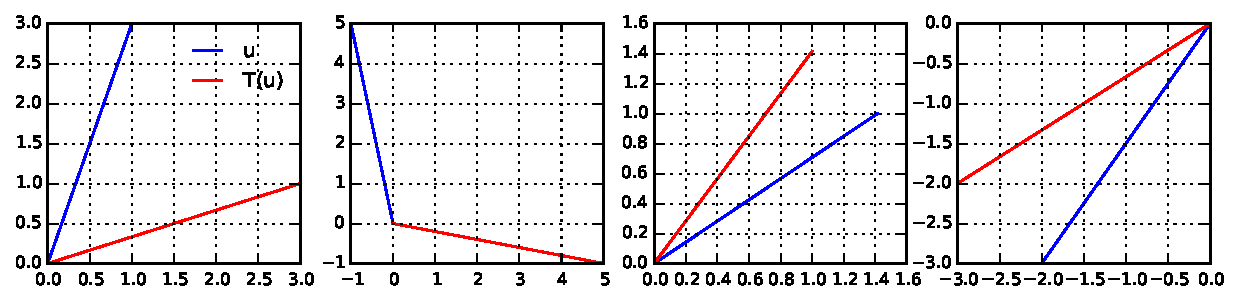
\includegraphics[width=1.2\linewidth]{figs/ex5_1_1a.pdf}

\subsubsection{Exercise 5.1.5}
%-----------------------------

Given the transformation (mapping) \ref{eq:ex5_1_5} in $\mathbb{R}^3$:

\begin{equation}\label{eq:ex5_1_5}
T{\left (\left[\begin{matrix}x\\y\\z\end{matrix}\right] \right )} =
\left[\begin{matrix}x + y\\
                    y + z\\
                    z + x\end{matrix}\right]
\end{equation}

determine whether the transformation \ref{eq:ex5_1_5} is linear.

In other words, we need to check whether the conditions \textbf{A} and
\textbf{B} above are satisfied.

First define a function with the transformation $T$ to be tested. Then define two generic
vectors \textbf{u} and \textbf{v} and see if applying $T$ satisfies the conditions
for linearity.

\begin{verbatim}
x, y, z, s, t, l, k= symbols('x y z s t l k', real= True)

def T(u):
    Tu= Matrix([u[0] + u[1],
                u[1] + u[2],
                u[2] + u[0]])
    return(Tu)
\end{verbatim}

Get two vectors and test conditions for linearity:

\begin{verbatim}
u= Matrix([x, y, z])
v= Matrix([s, t, l])

## Cond A:
assert (T(u + v)) - (T(u) + T(v)) == zeros(3, 1)

## Cond B:
assert (T(k * u) - k * T(u)).expand() == zeros(3, 1)
\end{verbatim}

Assertions return \texttt{True} hence the transformation \texttt{T} is linear.

Pay attention how the conditions for equality are tested in \sympy. We subtract
one term from the other and check the result is zero, in this case the zero vector
in $\mathbb{R}^3$ $[0\ 0\ 0]^T$. Using the double equal sign \texttt{==} would return
\texttt{False} in the second assertion since \texttt{==} tests for identity of form
not for \textbf{symbolic identity}. See also \href{https://github.com/sympy/sympy/wiki/Faq}{
Why does SymPy say that two equal expressions are unequal?}

The trasformation $T$:

$$
T(\left[\begin{matrix}x\\y\\z\end{matrix}\right]) = \left[\begin{matrix}\sqrt{x}\\\sqrt{y}\\\sqrt{z}\end{matrix}\right]
$$

Is not linear since $\sqrt{a + b} = \sqrt{a} + \sqrt{b}$ is not satisfied.

\begin{verbatim}
def T(u):
    Tu= Matrix([sqrt(u[0]), sqrt(u[1]), sqrt(u[2])])
    return(Tu)
    
u= Matrix([x, y, z])
v= Matrix([s, t, l])

## Cond A
(T(u + v)).expand() - (T(u) + T(v)).expand() == zeros(3, 1) ## False

## Cond B
(T(k * u)).expand() - (k * T(u)).expand() == zeros(3, 1) ## False
\end{verbatim}

\subsubsection{Exercise 5.1.6 a}
%-------------------------------

This is an helper function which might be useful elsewhere \footnote{See also
on StackOverflow \href{http://stackoverflow.com/questions/29434911/sympy-how-to-get-zero-for-absent-constant-term/}
{How to get zero for absent constant term.}}. Here we use it to implement the
tranformation \ref{eq:ex5_1_6a} where we need to swap the coefficients of a
polynomial. By returning a dictionary of terms and coefficients, \texttt{getCoeffDict}
makes the manipulation of coefficients easier.

\begin{equation}\label{eq:ex5_1_6a}
T(c_2 x^2 + c_1 x + c_0) = c_0 x^2 + c_1 x + c_2
\end{equation}

\begin{verbatim}
def getCoeffDict(exprs, x):
    """Return a dict of coefficients for each power of the variable `x` in
    expression `exprs`. Examples:
    
        >>> x, a, b, c= symbols('x a b c')
        >>> getCoeffDict(a*x**2 + b*x + c, x)
        {x**2: a, x: b, 1: c}
        >>> getCoeffDict(a*x**2, x)
        {1: 0, x: 0, x**2: a}
    """
    exprs= exprs.expand()
    n= Poly(exprs).degree(x)
    cdict= {}
    for i in range(0, n+1):
        cdict[x**i]= exprs.coeff(x, i)
    return(cdict)
\end{verbatim}

Let's proceede testing whether \ref{eq:ex5_1_6a} is a linear tranformation. Note
that the transformation \ref{eq:ex5_1_6a} works in polynomial space, not in
Euclidean space. However, the approach remains the same.

\begin{enumerate}
\item{Define the transformation of interest}
\begin{verbatim}
def T(p):
    k= getCoeffDict(p, x)
    Tp= k[1]*x**2 + k[x]*x + k[x**2]
    return(Tp)
\end{verbatim}

\item{Get two generic vectors:}
\begin{verbatim}
k= symbols('k', nonzero= True)
c0, c1, c2= symbols('c0 c1 c2')
b0, b1, b2= symbols('b0 b1 b2')

p= c2*x**2 + c1*x + c0
q= b2*x**2 + b1*x + b0
\end{verbatim}

\item Test condition $T(\mathbf{u + v}) = T(\mathbf{u}) + T(\mathbf{v})$
\begin{verbatim}
( (T(p+q)) - (T(p)+T(q)) ).expand() == 0 ## True
\end{verbatim}

\item Test condition $T(k\mathbf{u}) = kT(\mathbf{u})$
\begin{verbatim}
(T(k * p)) - (k * T(p)).expand() == 0 ## True
\end{verbatim}
\end{enumerate}

\subsubsection{Exercise 5.1.6 b}
%-------------------------------

Similar to \textit{a} above. For

$$
T(c_2 x^2 + c_1 x + c_0) = c_2^2 x^2 + c_1^2 x + c_0^2
$$

\begin{verbatim}
def T(p):
    k= getCoeffDict(p, x)
    Tp= k[x**2]**2 * x**2 + k[x]**2 * x + k[1]**2
    return(Tp)

p= c2*x**2 + c1*x + c0
q= b2*x**2 + b1*x + b0

# Is `kT(u) = T(ku)`?
((k*T(p)).expand() - (T(k*p)).expand()) == 0 # False
\end{verbatim}

Condition $T(k\mathbf{u}) = kT(\mathbf{u})$ can't be satisfied hence the
transformation is not linear.

$$
k \left(c_{0}^{2} + c_{1}^{2} x + c_{2}^{2} x^{2}\right) \neq c_{0}^{2} k^{2} + c_{1}^{2} k^{2} x + c_{2}^{2} k^{2} x^{2}
$$

\subsubsection{Exercise 5.1.7 a}
%-------------------------------

Check whether matrix transposition is a linear transformation. See \texttt{?Matrix.equals}
for testing matrix equality.

\begin{verbatim}
def T(A):
    return A.transpose()

a, b, c, d, e, f, g, h, i= symbols('a:i')
A= Matrix(2,2, [a,b,c,d])
B= Matrix(2,2, [f,g,h,i])

T(A+B).equals(T(A) + T(B)) ## True
(k*T(A)).equals(T(k*A))    ## True
\end{verbatim}

Matrix transposition \emph{is} linear.

Again, we are not working in Euclidean space but the approach is the same. This
is \emph{matrix space of size \emph{n} by \emph{n}}.

\subsubsection{Exercise 5.1.9}
%-------------------------------

Test whether \emph{integration} is linear. Note that integration maps from space
$C{0, 1}$ to $\mathbb{R}$.

\begin{verbatim}
f= Function('f')(x)
def T(f):
    return integrate(f, (x, 0, 1))
    
x= symbols('x', real= True, nonnegative= True, nonzero= False)
f= Function('f')(x)
g= Function('g')(x)

(T(f+g)).equals(T(f) + T(g)) ## Returns None
(k*T(f)).equals(T(k*f))  ## True
\end{verbatim}

First condition is satisified since:

$$
\int_{0}^{1} f{\left (x \right )} + g{\left (x \right )}\, dx = \int_{0}^{1} f{\left (x \right )}\, dx + \int_{0}^{1} g{\left (x \right )}\, dx
$$

\sympy returns \texttt{None} and this might be ok since \emph{$[$\texttt{Function.equals} returns$]$ None
(instead of T/F) for an expression that *is* zero but won't simplify to zero.}
(See \href{https://groups.google.com/forum/#!topic/sympy/xP_uM49pXeo}{\sympy discussion group})

\subsection{5.2 Kernel and range of a linear transformation}
% ==========================================================

The \textbf{kernel} of a linear transformation is the set of domain (starting)
values which map to zero in the codomain (arrival). \emph{I.e.} the kernel of
$T$ is:

$$
T(\mathbf{v}) = \mathbf{O})
$$

The \textbf{range} or \textbf{image} of a linear transformation is the
subset of values in the codomain $W$ where a linear transformation $T$ can arrive.
Formally:

$$
range(T) = {T(\mathbf{v}) | \mathbf{v} in V}
$$

\section{Appendix}
% ****************

\subsection{Plotting with \texttt{matplotlib.pyplot}}
% ===================================================

The documentation of \texttt{matplotlib} and its modules is quite extensive
but it doesn't give a simple overview of how graphics are organized. Therefore this
section outlines the idea behind \texttt{pyplot} graphics and its components. 

\cmd{pyplot} is a layer on \texttt{matplotlib} to provide graphic facilities
similar to Matlab. \texttt{pyplot} appears to be the preferred way to plot
graphics in \texttt{python/matplotlib}. See also \href{http://matplotlib.org/faq/usage_faq.html}{matplotlib usage} and 
the tutorial \href{https://github.com/ericliang/matplotlib/blob/master/trunk/scipy06/oo_resources/leftwich_tut.txt}
{Getting Started With Matplotlib}.

So, first import the \cmd{pyplot} module:

\begin{verbatim}
import matplotlib.pyplot as plt
\end{verbatim}

and get some dummy data to play with:

\begin{verbatim}
import numpy as np

x= np.array([1, 2, 3, 4])
y= x**2
\end{verbatim}

Here \texttt{x} and \texttt{y} are numpy arrays, although \texttt{pyplot} accepts
any iterable.

\subsubsection{Figure}
% --------------------------
\begin{verbatim}
fig= plt.figure()
\end{verbatim}

\cmd{matplotlib.figure.Figure()} is the top level of a graphics where everything starts
and it is therefore the equivalent of a blank sheet of paper where you draw the plot on. Use \texttt{figure}
to set among other things the \textbf{size} of the figure (in inches) and the \textbf{dpi} resolution,
if applicable. More or less the call \texttt{fig= plt.figure()} is equivalent to
\texttt{R}'s \texttt{g<- ggplot()}. \texttt{figure()} can be called with only default parameters;
in fact, a call to \texttt{Figure} can be skipped altogheter (see below). 

\subsubsection{Axis}
% ------------------

\begin{verbatim}
axes= fig.add_subplot(1, 3, 2)
\end{verbatim}

To draw on a \texttt{Figure} object you need to put a set of \cmd{Axes} where you actually
draw stuff.

\texttt{Axes} can be put with \cmd{.add\_subplot} or \cmd{.add\_axes}. \texttt{add\_subplot}
is similar to \texttt{R} \texttt{par(mfrow= c(n, m))} in that it divides the figure
in \emph{n} rows and \emph{m} columns. The third argument in \texttt{add\_subplot} states
which subplot should be drawn upon. \emph{E.g.} \texttt{fig.add\_subplot(1, 3, 2)}
sets one row, three columns, and draws in the middle subplot (number 2).

Alternatively \cmd{.add\_axes} can be used to specify the characteristics of the
plotting box. It's roughly equivalent to \texttt{R} \texttt{par(mar= c(a, b, c, d))}
in that you set the position of the axes relative to the overall figure. It can also
be used to add plot on top of each other, like figure insets.

The \cmd{Axes} object can be used to control graphic parameters like x- and y-limits,
the axis labels and the plot title. It controls more or less what you can control with \texttt{R}'s \texttt{par()}.

As for \texttt{Figure}, you can add a subplot with only default arguments or skip
the call altogether.

\subsubsection{Plotting}
% ----------------------

\begin{verbatim}
axes.plot(x, y)
\end{verbatim}

Drawing is realized by adding stuff to the \texttt{Axes} object, typically by means
of \cmd{plot()} function. Similar to \texttt{R plot()}, with \texttt{plot} you can
set the plotting style (line, point), colour, etc. See \href{http://matplotlib.org/api/pyplot_api.html#matplotlib.pyplot.plot}
{pyplot.plot} for documentation of setting line styles and plotting features.

\subsubsection{Rendering}
% ----------------------

\begin{verbatim}
fig.savefig('filename.pdf')
fig.show()
plt.close()
\end{verbatim}

The actual plot is visualized with the \cmd{show()} method and saved to file with
\cmd{savefig()} method. By default, file format is deduced from file extension.
Finally, call \cmd{close} to close the grahic device(s).

\subsubsection{In practice...}
% ----------------------------

In practice you can take shortcuts to create plots. It is not strictly necessary
to explicitly set up a \texttt{Figure} and \texttt{Axes} object.

\begin{verbatim}
plt.plot(x, y, 'r--', lw= 2)
plt.plot(x, y, 'bo', markersize=12)
plt.xlabel('x-lab')
plt.xlim([0, 5])
plt.rc('font', size= 20)
plt.grid()
plt.savefig('figs/app_simple.pdf', bbox_inches= 'tight')
plt.show()
\end{verbatim}

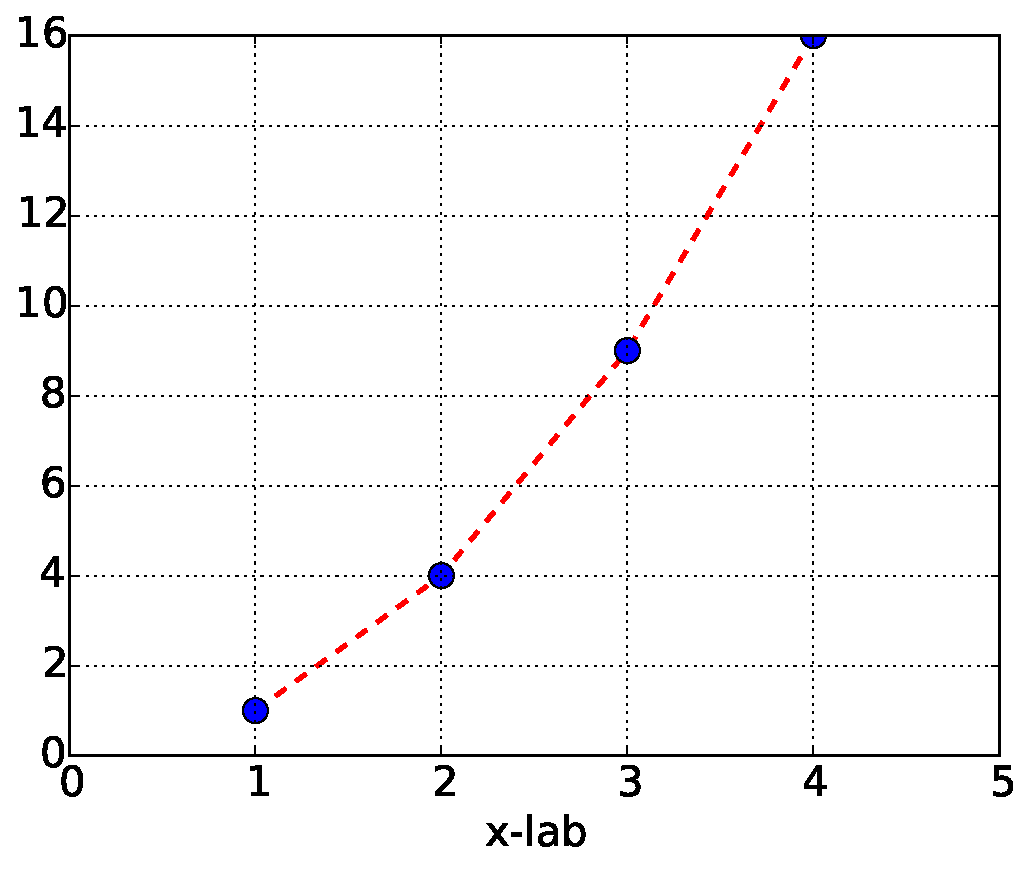
\includegraphics[width=0.5\linewidth]{figs/app_simple.pdf}

For simple plots, you can just call \cmd{plt.plot()} with the data to plot and
optional graphic paramaters. The bare minimum to see an xy-plot is just
\texttt{plt.plot(x, y); plt.show()}

Note that you keep adding features using \texttt{plt.<feature>},
then when you call \texttt{savefig} or \texttt{show} everything comes together.
In contrast to \texttt{R}, the order with which you add these features doesn't
matter. However, if you want to save to file \emph{and} show on screen, remember
to call \texttt{savefig} first and \texttt{show} then.

\begin{verbatim}
plt.rc('font', size= 8)
fig, axlst = plt.subplots(1, 3, sharex=True, sharey= True)
axlst[0].plot(x, y)
axlst[1].plot(x, y*2)
axlst[2].plot(x, y*3)
fig.subplots_adjust(wspace= 0.1)
fig.set_size_inches(18/2.54, 6/2.54)
fig.savefig('figs/app_subplot.pdf')
fig.show()
\end{verbatim}

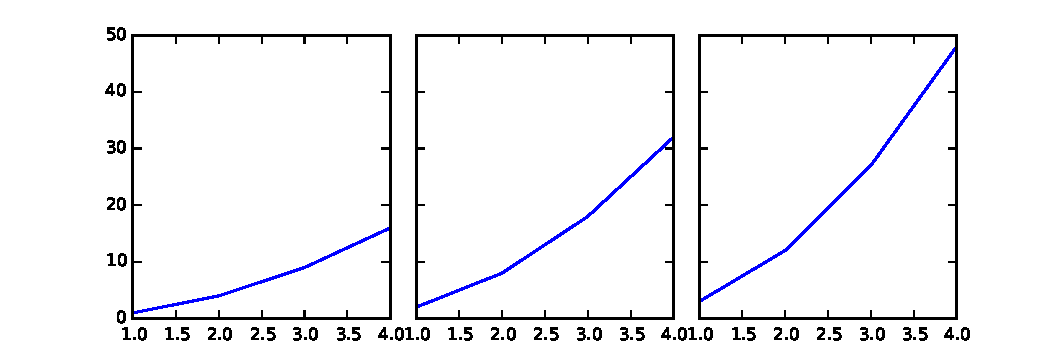
\includegraphics[width=\linewidth]{figs/app_subplot.pdf}

For multiple plots it might be best to set up the \texttt{Figure} object and the
list (array actually) of subplots in one call to \cmd{plt.subplots()}. Each element
of the array contains an \texttt{Axes} object that can be individually populated.
The \texttt{Axes}'s can be juxtaposed by playing with the method \cmd{Figure.subplots\_adjust}.
For example to set the spacing. 

\subsubsection{Example}
% ---------------------

\begin{verbatim}

fig= plt.figure()
ax1= fig.add_subplot(1, 3, 1)
ax1.plot(x, y, 'r--')
ax2= fig.add_subplot(1, 3, 2)
ax2.plot(x, y, 'pg')
ax3= fig.add_subplot(1, 3, 3)
ax3.plot(x, y, 'p')
for i, txt in enumerate(x):
    ax3.annotate(txt, (x[i], y[i]))
fig.show()
\end{verbatim}

\subsection{Principal components}
% ===============================

\dots

For interpretation of eigenvalues and eigenvectors of a covariance matrix see
http://www.visiondummy.com/2014/04/geometric-interpretation-covariance-matrix/

\subsection{PageRank}
% ===================

Google ranks pages predominantly according to two criteria: 1) Number of links a page
receives, \emph{i.e.} many other pages rerfers to it, or in other words it is 'cited' very often;
2) Incoming links are not all equal, incoming links from important pages are more
important, \emph{i.e.} being 'cited' by a very important page counts more.

See also \href{http://www.math.cornell.edu/~mec/Winter2009/RalucaRemus/Lecture3/lecture3.html}{The Mathematics of Google Search}

Stochastic matrix, \textit{i.e.} where column sums equal 1, describing how node weights
are distibuted.

\begin{equation}
\mathbf{A} = \left[\begin{matrix}0 & 0 & 1.0 & 0.5\\0.3 & 0 & 0 & 0\\0.3 & 0.5 & 0 & 0.5\\0.3 & 0.5 & 0 & 0\end{matrix}\right]
\end{equation}

\begin{itemize}
\item Each \textbf{column} describes how each node distributes its weight.

For example, $1^{st}$ column, $[0\ \frac{1}{3}\ \frac{1}{3}\ \frac{1}{3}]^T$, says that node $x_1$ gives 0 of its
weight to itself (of course), 1/3 to $x_2$, 1/3 to $x_3$, and 1/3 to $x_4$;
$4^{th}$ column describes node $x_4$ and it says that 1/2 weight is given to $x_1$,
0 to $x_2$, 1/2 to $x_3$, and 0 to itself.

\item Each \textbf{row} describes the weight or score of each node, since it is the SUM
of all the node weights.

For example, $1st$ row is the score for node $x_1$. $x_1$
receives 0 from itself (of course), 0 of the weight of $x_2$, 1 (\textit{i.e. all})
of the weight from $x_3$, and 1/2 of the weight from $x_4$.
\end{itemize}

So matrix \textbf{A} tells the \textit{proportion} of weight to and from nodes. The question
is: \emph{How much each node weighs?} If all the nodes had the same weight the row sums
of \textbf{A} would give the page rank already. However, we want to give more weight
to pages that have many incoming links and/or incoming links from high ranking pages.
For example, node $x_1$ receives all of the weight from $x_3$ (1) and half of the weight
from $x_4$ (0.5). But how much do $x_3$ and $x_4$ weigh?

The assign weights to nodes we need to solve the linear system where the LHS is
matrix \textbf{A} and RHS is the vector of weights (ranks) we want to find out:

\begin{equation}
\left[\begin{matrix}
0 x_1 + 0 x_2 + 1 x_{3} + 0.5 x_{4} \\
0.3 x_{1}  + 0 x_2 + 0 x_3 + 0 x_4 \\
0.3 x_{1} + 0.5 x_{2} + 0 x_3 + 0.5 x_{4} \\
0.3 x_{1} + 0.5 x_{2} + 0 x_3 + 0 x_4
\end{matrix}\right] =
\left[\begin{matrix}x_{1}\\ x_{2}\\x_{3}\\x_{4}\end{matrix}\right]
\end{equation}

This is equivalent to finding the eigenvector of \textbf{A} for the eigenvalue 1.
In fact see that if we set $\left[\begin{matrix}x_{1}\\x_{2}\\x_{3}\\x_{4}\end{matrix}\right] = \mathbf{u}$,
we have in matrix notation:

\begin{equation}
\mathbf{Au = \lambda u}; \quad and\ for\ \lambda = 1: \quad \mathbf{Au = u}; 
\end{equation}

which is the definition of eigenvectors/values. Note that since \textbf{A} is
stochastic the largest eigenvalue is always 1 \footnote{see also
\href{http://math.stackexchange.com/questions/40320/proof-that-the-largest-eigenvalue-of-a-stochastic-matrix-is-1}
{proof that the largest eigenvalue of a stochastic matrix} on Math Stack Exchange.}.

In this example the eigenvector for $\lambda = 1$ is $\mathbf{u} = \left[\begin{matrix}1\\0.33\\0.75\\0.5\end{matrix}\right]$.
We can normalize the scores to sum to 1 and obtain the pageRank
$PR =
\left[\begin{matrix}x_{1}\\x_{2}\\x_{3}\\x_{4}\end{matrix}\right] =
\left[\begin{matrix}0.39\\0.13\\0.29\\0.19\end{matrix}\right]$

Represent the web as a grpah and implement it as a dictionary of dictionaries. The outer dictionary has pages
(nodes) as keys. The value of each key (page) is a dictionary of outgoing links.
This inner dictionary has key: The arraival page, value: The weight transferred to
that page.

\begin{verbatim}
graph= {
    1: {2: 0, 3: 0, 4: 0},
    2: {3: 0, 4: 0},
    3: {1: 0},
    4: {1: 0, 3: 0}
}

# Assign weights to pages. Outgoing links:
for p in graph:
    pout= graph[p]
    for w in pout:
        pout[w]= 1.0 / len(pout)

# Matrix representation
pages= sorted(graph.keys())
A= np.array(zeros(len(pages), len(pages)))
for ci in range(len(pages)):
    page= graph[pages[ci]]
    for ri in range(len(pages)):
        outk= pages[ri]
        if outk in page:
            A[ri][ci]= page[outk]
A= Matrix(A)

# Solve A * u = u in order to get the ranks u:
u= Matrix(symbols('x1:%s' %(A.cols+1)))
Au= Eq(A*u, u)
sols= solve(Au.subs(x1, 1), u[1:])
sols[x1]= 1

# Or get all eigenvects, but slower since it calculates all of them:
A.eigenvects()[0]

# Normalize ranks to sum to 1
s= sum(sols.values())
pageRank= {}
for x in sols:
    pageRank[x]= sols[x]/s

PR= Matrix([pageRank[x] for x in u])

# Test we did it right
Eq(A * PR, PR) # True

\end{verbatim}

What if a page has no outgoing links? For example
\footnote{From J. Hefferon - Linear Algebra, Topic: Page Ranking}, in this graph
page 4 has no outgoing links:

\begin{verbatim}
graph= {
    1: {2:0},
    2: {3: 0},
    3: {1: 0, 2: 0, 4: 0},
    4: {}
}
\end{verbatim}

In this case we can imaging that a surfer reaching page 4 will move at random to
any other page. \emph{I.e.} we distribute the weight of page 4 uniformaly across
all the other pages:

\begin{verbatim}
for p in graph:
    pout= graph[p]
    if pout == {}:
        # If a page has no outgoing links distribute its weight across all web 
        for x in graph:
            graph[p][x]= 1.0 / len(graph)
    else:
        for w in pout:
            pout[w]= 1.0 / len(pout)
        graph[p]= pout
\end{verbatim}

This web looks like:

\begin{verbatim}
graph= 
{1: {2: 1.0},
 2: {3: 1.0},
 3: {1: 0.33, 2: 0.33, 4: 0.33},
 4: {1: 0.25, 2: 0.25, 3: 0.25, 4: 0.25}}
\end{verbatim}

As above, transform the graph in a stochastic matrix:

$$
\mathbf{A} = \left[\begin{matrix}0 & 0 & 0.33 & 0.25\\1.0 & 0 & 0.33 & 0.25\\0 & 1.0 & 0 & 0.25\\0 & 0 & 0.33 & 0.25\end{matrix}\right]
$$

\begin{verbatim}
pages= sorted(graph.keys())
A= np.array(zeros(len(pages), len(pages)))
for ci in range(len(pages)):
    page= graph[pages[ci]]
    for ri in range(len(pages)):
        outk= pages[ri]
        if outk in page:
            A[ri][ci]= page[outk]
A= Matrix(A)
\end{verbatim}

Obtain eigenvector for $\lambda= 1$ and normalize to have ranks to sum to 1
$$
PR = \left[\begin{matrix}0.16\\0.32\\0.36\\0.16\end{matrix}\right]
$$

Remember that there is an infinite number of eigenvectors belonging to an eigenvalue.
In fact we talk about \emph{eigenspace}. For convenience we choose the eigenvector
whose sum is 1.

\begin{verbatim}
def rankMatrix(A):
    """Return page ranks for matrix of weights A"""
    u= Matrix(symbols('x1:%s' %(A.cols+1)))
    Au= Eq(A*u, u)
    Au= Au.subs(x1, 1) # This sub is arbitrary, any real will do.
    sols= solve(Au, u[1:])
    sols[x1]= 1
    
    s= sum(sols.values())
    pageRank= {}
    for x in sols:
        pageRank[x]= sols[x]/s
    PR= Matrix([pageRank[x] for x in u])
    return PR
\end{verbatim}

Google edits the page rank matrix \textbf{A} to add some randomess in the behaviour
of the surfer. That is, a surfer every now and then might jump to a page not linked
in to the current one. The probability of jumping to an unlinked page is $\alpha$,
typically between 0.85 and 0.99.
To model this behaviour we edit the weight matrix \textbf{A} as follow:

\begin{itemize}
\item Edit the weights in weight matrix \textbf{A} by multiplying by the correction
factor $\alpha$, $\mathbf{A_{rnd}} = \alpha \mathbf{A}$.

\item Add to the corrected matrix $\alpha\mathbf{A}$ weights so that it returns to
be stochastic, \emph{i.e.} add $(1 - \alpha) \mathbf{R}$ where \textbf{R} is a matrix
of the same dim as \textbf{A} and with column sums 1.
\end{itemize}

Putting it all together, we obtain the \emph{Google matrix} \textbf{G} with the \emph{linear
combination}:

$$
\mathbf{G} = \alpha \mathbf{A} + (1 - \alpha) \mathbf{R}
$$

For this example:

$$
\mathbf{G} =
\alpha \left[\begin{matrix}0 & 0 & 0.33 & 0.25\\1.0 & 0 & 0.33 & 0.25\\0 & 1.0 & 0 & 0.25\\0 & 0 & 0.33 & 0.25\end{matrix}\right] +
(1 - \alpha) \left[\begin{matrix}0.25 & 0.25 & 0.25 & 0.25\\0.25 & 0.25 & 0.25 & 0.25\\0.25 & 0.25 & 0.25 & 0.25\\0.25 & 0.25 & 0.25 & 0.25\end{matrix}\right] =
$$

$$
\left[\begin{matrix}0 & 0 & 0.28 & 0.2125\\0.85 & 0 & 0.28 & 0.2125\\0 & 0.85 & 0 & 0.2125\\0 & 0 & 0.28 & 0.2125\end{matrix}\right] +
\left[\begin{matrix}0.0375 & 0.0375 & 0.0375 & 0.0375\\0.0375 & 0.0375 & 0.0375 & 0.0375\\0.0375 & 0.0375 & 0.0375 & 0.0375\\0.0375 & 0.0375 & 0.0375 & 0.0375\end{matrix}\right] =
\left[\begin{matrix}0.0375 & 0.0375 & 0.32 & 0.25\\0.8875 & 0.0375 & 0.32 & 0.25\\0.0375 & 0.8875 & 0.0375 & 0.25\\0.0375 & 0.0375 & 0.32 & 0.25\end{matrix}\right]
$$

The page ranks now become $PR_{\alpha=0.85} = \left[\begin{matrix}0.17 \\0.36 \\0.34 \\0.17 \end{matrix}\right]$.

Note that if $\alpha = 1$ than there is no randomess at all. If $\alpha = 0$ instead
the surfing is complete random and the page ranks become $PR_{\alpha=1} = \left[\begin{matrix}0.25\\0.25\\0.25\\0.25\end{matrix}\right]$

\begin{verbatim}
def googleRank(A, alpha= 0.85):
    """Ranks pages in weight matrix A after having add some random surfing
    behaviour alpha"""
    R= Matrix(A.rows, A.cols, [1/A.cols] * A.rows * A.cols)
    G = alpha * A + (1 - alpha) * R
    PR= rankMatrix(G)
    return PR

googleRank(A, 0.85)
\end{verbatim}

\subsection{Line of best fit (least squares)}
% ===========================================

\dots


\end{document}
